%========================= Classe du Document ==========================
\documentclass[a4paper,fleqn,12pt,openright]{report}
%============================= Packages ================================
\usepackage[T1]{fontenc}
\usepackage[hidelinks]{hyperref} % Cick on citations
\usepackage[utf8]{inputenc}
\usepackage[skip=10pt, indent=40pt]{parskip}  % Paragraph spacing
\usepackage{setspace} % Line spacing
\usepackage{caption}
\usepackage{subcaption} % Subcaptions for multiple figures 
\usepackage{multicol}

\usepackage{amsmath}
\usepackage{amssymb}
\usepackage{amsfonts}
\usepackage{amsthm}

\usepackage[margin=2.5cm]{geometry}
\usepackage{graphicx}
\usepackage{pgfplots}
\pgfplotsset{compat=1.18}
\usepackage{tikz}

\usepackage{xcolor}
\usepackage{xspace} % For \onedot command

\usepackage[acronym, toc]{glossaries}
\usepackage{breakcites} % Citations over multiple lines

%\setlength{\parindent}{0pt}  % Paragraph indentation 

%Import the natbib package and sets a bibliography  and citation styles
\bibliographystyle{apalike}

%=============================== Commands ===================================

\newcommand{\comseb}[1]{{\color{red}SEB: \textit{#1}}}
\newcommand{\comroman}[1]{{\color{purple}ROMAN: \textit{#1}}}
\newcommand{\commanu}[1]{{\color{green}MANU: \textit{#1}}}
\newcommand{\commanue}[1]{{\color{cyan}MANUE: \textit{#1}}}
\newcommand{\comloic}[1]{{\color{orange}LOIC: \textit{#1}}}

\newcommand{\M}{{\mathfrak{M}}}
\newcommand{\X}{{\mathcal{X}}}
\newcommand{\low}{{\underline{P}}}
\newcommand{\tdt}{{\times\dots\times}}
\newcommand{\opi}{{[\![}}
\newcommand{\cli}{{]\!]}}



\newtheorem{theorem}{Theorem}[section]
\theoremstyle{definition}
\newtheorem{example}{Example}[section]
\newtheorem{proposition}{Proposition}[section]
\newtheorem{definition}{Definition}[section]
\newtheorem{remark}{Remark}[section]

% From CVPR cvpr.sty
\makeatletter
\DeclareRobustCommand\onedot{\futurelet\@let@token\@onedot}
\def\@onedot{\ifx\@let@token.\else.\null\fi\xspace}

\def\eg{\emph{e.g}\onedot} \def\Eg{\emph{E.g}\onedot}
\def\ie{\emph{i.e}\onedot} \def\Ie{\emph{I.e}\onedot}
\def\cf{\emph{cf}\onedot} \def\Cf{\emph{Cf}\onedot}
\def\etc{\emph{etc}\onedot} \def\vs{\emph{vs}\onedot}
\def\st{\emph{s.t}\onedot}
\def\wrt{w.r.t\onedot} \def\dof{d.o.f\onedot}
\def\iid{i.i.d\onedot} \def\wolog{w.l.o.g\onedot}
\def\etal{\emph{et al}\onedot}
\makeatother
%========================= Glossary ====================================

\makeglossaries
\newglossaryentry{EO}
{%
    name={Earth Observation},
    description={Earth Observation involves employing remote sensing techniques for terrestrial, marine, and atmospheric monitoring}
}

\newglossaryentry{DISPARITY}
{%
    name={Disparity},
    description={The displacement of an object between two stereo images when expressed in pixels}
}

\newglossaryentry{DSM}
{%
    name=Digital Surface Model,
    description={Representation of the elevation of an area using a raster, including the vegetation, buildings \etc. Also called Digital Elevation Model. Sometimes referred to as a 2.5D model, as it is a 2D grid where each cell contains data about the elevation}
}

\newglossaryentry{DTM}
{%
    name={Digital Terrain Model},
    description={Representation of the terrain of an area using a raster, excluding the vegetation and buildings}
}

\newglossaryentry{LiDAR}
{%
    name={Light Detection And Ranging},
    description={Sometimes referred to as Laser Imaging Detection And Ranging. A LiDAR is an active sensor allowing to determine the distance between the sensor and its surroundings by measure the time between the emission of a laser beam and the detection of its reflection on the environment}
}

\newglossaryentry{Panchromatic}
{%
    name={Panchromatic image},
    description={A panchromatic image is an image representing the light in the visible spectrum, resulting in a black and white image. Satellites equipped with panchromatic sensors usually produce images of higher resolution than classical RGB sensors, although a high resolution RGB image can be obtained from a panchromatic image using a method called pansharpening}
}
\newacronym{b/h}{B/H}{Base-to-Height ratio}
\newacronym{cnes}{CNES}{Centre National d'Etudes Spatiales}
\newacronym{co3d}{CO3D}{Constellation Optique 3D}
\newacronym{dem}{DEM}{Digital Elevation Models}
\newacronym{dsm}{DSM}{Digital Surface Model}
\newacronym{dtm}{DTM}{Digital Terrain Model}
\newacronym{gis}{GIS}{Geographic Information Systems}
\newacronym{nir}{NIR}{Near Infra Red}
\newacronym{rgb}{RGB}{Red Green Blue}
\newacronym{vhr}{VHR}{Very High Resolution}
\newacronym{eo}{EO}{Earth Observation}
\newacronym{lidar}{LiDAR}{Light Detection And Ranging}
\newacronym{rpc}{RPC}{Rational Polynomial Models}


\pdfstringdefDisableCommands{%
  \def\glspl#1{<#1>}} % To silence hyperref Warning Token not allowed in a PDF string (Unicode)
%=======================================================================
%=======================================================================

\begin{document}

\definecolor{color}{HTML}{F5F5F5}
%======================= Page de Garde =================================
\thispagestyle{empty}
\begin{titlepage}
    \begin{center}
        \Huge
        \textbf{Uncertainty characterisation in stereophotogrammetry using satellite images}
            
        \vspace{0.5cm}
        \LARGE
        Caractérisation d'incertitude pour la stéréophotogrammétrie à partir d'images satellites

        \vspace{1.cm}
        \large
        Defended by\\
        \textbf{Roman MALINOWSKI}\\
        \vspace{0.8cm}
        Members of the jury\\
        
        \vspace{0.2cm}
        President: \textbf{Benjamin QUOST}\\
        Reviewers: \textbf{Isabelle BLOCH}, \textbf{Marc PIERROT DESEILLIGNY}\\
        External members: \textbf{Luc JAULIN}, \textbf{Olivier STRAUSS}\\
        Supervisors: \textbf{Sébastien DESTERCKE}, \textbf{Emmanuel DUBOIS}, \textbf{Loïc DUMAS}, \textbf{Emmanuelle SARRAZIN}\\
    
        \vspace{1cm}
        Speciality: Sciences et Technologie de l'Information et de la Communication\\~\\
        Centre National D'Etudes Spatiales - CS Group \\
        Heudiasyc, Université de Technologie de Compiègne\\
        ~\\
        19/12/2024
        \
        \begin{figure}[hb]
            \begin{subfigure}[b]{0.3\linewidth}
                \centering
                \includegraphics[height=2.5cm]{Images/General/Logo_CNES.png}
            \end{subfigure}\hfill
            \begin{subfigure}[b]{0.3\linewidth}
                \centering
                \includegraphics[height=1.5cm]{Images/General/Logo_CS.png}
            \end{subfigure}
        \end{figure}
        \begin{figure}
            \begin{subfigure}[b]{0.3\linewidth}
                \centering
                \includegraphics[height=1.3cm]{Images/General/Logo_UTC.jpg}
            \end{subfigure}\hfill
            \begin{subfigure}[b]{0.3\linewidth}
                \centering
                \includegraphics[height=1.3cm]{Images/General/Logo Région HDF - partenaire.jpg}
            \end{subfigure}
        \end{figure}
    \end{center}
\end{titlepage}


%==================== Glossaire, TOC etc ===============================
\tableofcontents
\thispagestyle{empty}
\pagebreak
\glsaddall
\pagenumbering{Alph}  % Switch Numerotation of pages to uppercase letters
\setcounter{page}{0}  % Resetting the page number
\printglossary[type=\acronymtype,nonumberlist]
\printglossary[nonumberlist]
\pagebreak

%========================== Les choses sérieuses commencent ===========

\pagenumbering{arabic}  % Switch numerotation of pages to Arabic
%\doublespacing
\onehalfspace

\addcontentsline{toc}{chapter}{Introduction}
\chapter*{Introduction}
\todoroman{Mettre le logo de la region Picardie sur la thèse}
\todoroman{Mettre un reading guide pour dire quel ``niveau d'expertise'' il faut en fonction des chapitres }
\pagebreak

\chapter{Introduction to Stereophotogrammetry}
\todoroman{TODO: Prendre le lecteur par la main, lui expliquer ce qu'il va lire et pourquoi dans cet ordre là \etc. Biblio sur la photogrammetry, l'utilité des DSM, la description des pipelines de photogrammetry, uncertainty dans les DSM.}

\todoroman{Mettre plus d'exemples, ou mieux le détailler}

\section{Digital Surface Models}
\todoroman{Utiliser les slides de formation CARS pour montrer les différentes méthodes pour faire de la 3D, mettre des exmples de LiDAR ou faire un schéma ?}

Knowing the Earth's topography is crucial for modern geosciences. As such, \acrfull{dsm}, which are a representation of a surface's elevation on a regular grid, appear as a natural solution in many \acrfull{gis}. Indeed, they can easily be handled and provide georeferenced information regarding the topography of an area. \acrshort{dsm} find usage in various contexts for a wide range of applications. In \acrfull{eo} for instance, \acrshort{dsm} are used to monitor changes in vegetation \cite{sadeghi_canopy_2016}, melting rates of glaciers \cite{berthier_glacier_2014, rieg_pleiades_2018}, volcanos \cite{ganci_data_2022}, snow or water resources \cite{marti_mapping_2016, yamazaki_merit_2019} \etc Similarly, \acrshort{dsm} are employed for catastrophe management, to predict the potential damage caused by earthquakes or floods \cite{jenkins_physics-based_2023} \dots \acrshort{dsm} are also crucial for ortho-rectifying image, \ie geometrically correcting the effects of distortions between the sensor and the terrain. This process creates a planimetric image with a consistent scale in all parts of the image. It allows images to be easily used in GIS or as background for maps. In urban settings, high resolution \acrshort{dsm} can help drone navigation for Defense applications, or more broadly for urban planning \cite{velazco_3d_2012}.

Nowadays, \acrshort{dsm} are mostly generated from laser scanning with LiDAR sensors, radar interferometry or stereophotogrammetry \cite{youssefi_cars_2020}. Air-borne laser scanning results in \acrfull{vhr} models, but the swath width and cost of acquisition campaigns do not allow to periodically cover the globe. Space-borne \acrshort{lidar} is mostly used for atmospheric measurements, or discrete measurements \cite{fouladinejad_history_2019} \todoroman{Et parler de ICESAT-2}. Space-borne radar interferometry remains widely used, and has allowed to create a worldwide digital model of emerged surfaces of the Earth at $30$m and $90$m resolution with the SRTM mission \cite{farr_shuttle_2007}. To obtain coarser resolutions, it is possible to leverage the technological advancement of optical sensors in orbit to create sub-meter \acrshort{dsm} using stereophotogrammetry with relatively low cost. However, this process is more complex than laser measurements as it deduces height from the principle of parallax. Stereophotogrammetry pipelines usually consists in multiple processing steps with intermediary products (see \ref{sec:classical_stero_pipeline}), with different methods, parameterization and post-processes available for each step (\eg matching, filtering \etc). This broad range of solutions allow to adapt our processes to the type of images and terrain observed, but it sometimes makes it difficult to determine the configuration producing the best quality DSM, or to single out a general good-working configuration. 

This thesis focuses on \acrshort{dsm} obtained from stereophotogrammetry, however we will use \acrshort{dsm} obtained from air-borne LiDAR acquisitions as references to validate our results, considering their high resolutions.

\todoroman{Schema de \acrshort{dsm} par avion LiDAR, satellite interfero et stereo}
\section{CO3D mission and Pléiades Satellites}
The following paragraphs detail satellites characteristics relevant to stereophotogrammetry. It is important to notice that although the sensor used greatly determines the resolution of the final \acrshort{dsm}, it is not the only factor at stake here. The altitude and positions of the satellites are also crucial for the resolution, and can be characterized by the \acrfull{b/h} \todoroman{Schema de \acrshort{dsm} par stereo avec le ratio B/H}. This ratio is computed by dividing the distance separating the stereo acquisitions by the altitude of the satellite. It indicates the angle formed between the line of sights originating from the satellites towards an object of the scene. A high \acrshort{b/h} allows for high elevation accuracy, but possesses more occluded regions (for instance a narrow street between two high buildings), and conversely for a low B/H \cite{delon_small_2007}.

The main source of images used in this thesis comes from Pléiades images. The Pléiades constellation developed by Airbus is composed of two identical satellites, 1A and 1B. The satellites were launched in 2011 and 2012 in an heliosynchronous orbit at $690$km, for both civilian and defense usages. They provide panchromatic images at a resolution of $70$cm (resampled at $50$cm), and RGB-NIR images at a resolution of $2$m, with a $20$km swath (\url{https://dinamis.data-terra.org/pleiades/}). Their high agility and revisit rate allow them to capture stereo and tri-stereo images for any location on the globe, ideal to produce \acrshort{dsm} with high accuracy. The \acrshort{b/h} ratio for stereo acquisitions can vary between $0.1$ and $0.4$. However, stereo acquisitions is not the only objective of this mission, even though the demand for those products is increasing \cite{berthier_glacier_2014, poli_radiometric_2015, rieg_pleiades_2018, loghin_potential_2020}. The acquisition of stereo images is thus provided on command, which can conflict with other usages of the satellite, and can become costly when trying to cover large areas.  
\begin{figure}
    \centering
    \begin{subfigure}{0.5\linewidth}
        \centering
        \includegraphics[height=6cm]{Images/Chap_1/Paris_003.jpeg}
        \caption{$14/10/2017$ $11:03:003$}
        \label{fig:Pleiade_over_Paris_a}
    \end{subfigure}\hfill
    \begin{subfigure}{0.5\linewidth}
        \centering
        \includegraphics[height=6cm]{Images/Chap_1/Paris_403.jpeg}
        \caption{$14/10/2017$ $11:03:403$}
        \label{fig:Pleiade_over_Paris_b}
    \end{subfigure}
    \caption{Pansharpened Pléiades stereo images over Paris at $0.5$m of resolution. Pléiades \copyright CNES 2017, Distribution AIRBUS DS}
    \label{fig:Pleiade_over_Paris}
\end{figure}

In order to produce a worldwide \acrshort{dsm} with $1$m resolution by 2025, the \acrfull{cnes} is launching the \acrfull{co3d} mission \cite{melet_co3d_2020}. Composed of two pairs of low-cost satellites equipped with \acrshort{vhr} optical sensors, the mission will produce image in the \acrshort{rgb} and \acrshort{nir} spectrum at $0.5$m of resolution \cite{lebegue_co3d_2020}. The pairing of satellites allows for \textit{almost} simultaneous stereo image acquisition, cutting short the transient object problem (\ie objects moving/disappearing between stereo images). Different acquisition schemes can also be used, such as the video mode, or even the `diamond' geometry acquisition, which acquires a quadri-stereo over a couple of days. Depending on the relief of the terrain observed, the \acrshort{b/h} ratio will be between $0.2$ and $0.3$. In parallel with image quality specifications, the CO3D products need to abide to a height accuracy of $1$m on low slopes \comloic{à vérifier je crois que c'est 1m en relatif à CE90. En absolu je ne sais plus}. Another requirement, which is particularly relevant in the context of this thesis, is the production of a performance map supporting the output \acrshort{dsm}. Investigating sources and propagation of the uncertainty inside a 3D stereo pipeline can be beneficial for this performance map requirement. 

\todoroman{Parler de Maxar avec les Worldview ?}

\todoroman{Schema de la mission CO3D. Type of sensor, push-broom vs raster for CO3D}

One a side note, when an image is acquired both in panchromatic and RGB mode, it is possible to leverage the high resolution of the panchromatic image to improve that of the color image. This fusion technique is called \textit{pansharpening} \cite{loncan_hyperspectral_2015}. We use this technique for clarity in figures and other illustrations of this thesis. It is important to remember that the processed images are the panchromatic images, and not the pansharpened ones which are only used for the final visualization.

\section{Sensors and Georegistration}
Different types of sensors can be used to acquire satellite images. Below is detailed a (non-exhaustive) list of sensors of interest \cite{cnes_imagerie_2008}

\textbf{CCD matrix sensor}. CDD are classical sensors used, for instance, in current digital cameras. They possess multiple advantages, such as good geometrical quality as all pixels are acquired simultaneously, or the possibility to perform many acquisitions with various angles possible. However, CCD sensors with small pixel sizes are technologically difficult to built. Augmenting the number of pixels complicates the shutter function, and requires more radiometric calibration as one pixel equals one sensor. It is also more complex to acquire long segments of an image. CO3D satellites will use this technology.

\textbf{Push-broom sensor}. Those image sensors are only composed of a single cell row, acquiring simultaneously radiometric information alongside a line perpendicular to the direction of the satellite. As only one line of cells is needed, push-broom sensors are simple systems which can capture images continuously, while guarantying good geometrical quality along the rows of the images. A variation of those sensors are TDI sensors (Time Delay Integration). Those sensors function as a push-broom except that each row has the ability to transfer its photon charges to the next row. This allows to capture signals over a longer period of time,  thus reducing the signal-to-noise ratio. Harder to produce, TDI sensors also require a precise control of the satellite so that observed objects stay within a column of the TDI sensor. They are used in Pléiades satellites for instance.

\todoroman{Parler de l'incertitude des RPC, peut être dans une autre partie ? Et dire dans le scope of this PhD qu'on regarde pas cette incertitude. Regarder "Developement and Implementation of Rational Polynomial Coefficient Algorithms for Georeferencing Cartosat-1 Data", et "Metric Information Extraction from Spot Images and the Role of Polynomial Mapping Functions" de Baltsavias et Stallmann}
A crucial part of satellite imagery is the ability to perform georeferencement, or georegistratation, of every pixel, \ie, locate their coordinates in an Earth system of coordinates such as latitude and longitude. Physical models possess high localisation accuracy, but are sensor-specific and are computationally complex. For stereo reconstruction,  generalized sensor models are preferred. Specifically, we will focus on \acrfull{rpc} \cite{grodecki_ikonos_2001} used by the \acrshort{co3d} and Pléiades satellites. \acrshort{rpc} models are provided alongside images. Sometimes called Rational Function Models \cite{tao_comprehensive_2001}, \acrshort{rpc} are functions allowing to transform a pixel's ground location $(X,Y,Z)$ into its image coordinates $(row, col)$. \acrshort{rpc} encode the line of sight of the satellite, \ie the line joining the center of the sensor's cell to the ground and going through the optical center of the sensor. To improve numerical stability and minimize computation errors, the image coordinates and ground coordinates are normalized between $-1$ and $1$, using their scale factors $SF$ and mean values:
\begin{eqnarray*}
    SF_X &=& \max(X_\mathrm{max}-\overline{X},~\overline{X}-X_\mathrm{min})\\
    \Tilde{X}&=&\frac{X-\overline{X}}{SF_X}
\end{eqnarray*}
The same processed is applied to $Y,Z,row$ and $col$. To avoid heavy notation in this section, we will refer to every normalized coordinate using their non-normalized symbol.

\begin{figure}
    \centering
    \includegraphics[width=0.8\linewidth]{Images/Chap_1/RPC.png}
    \caption{Triangulation of the position of a point using RPC models\todoroman{Mettre les maisons en transoarent sur l'image?}}
    \label{fig:RPC}
\end{figure}

Formally, \acrshort{rpc} are defined as rational fractions of polynomials:  
\begin{eqnarray*}
    \mathrm{RPC}:\mathbb{R}^3 &\rightarrow&\mathbb{R}^2\\
    (X,Y,Z) 	&\mapsto& \left(\frac{Num_{row}(X,Y,Z)}{Den_{row}(X,Y,Z)}, \frac{Num_{col}(X,Y,Z)}{Den_{col}(X,Y,Z)}\right)\\
    &\mapsto&(row,col)
\end{eqnarray*}
where $Num_{row},~Den_{row},~Num_{col}$ and $Den_{col}$ are the numerators and denominators for rows and columns respectively, expressed as polynomials with a maximum order of $3$:
\begin{eqnarray*}
    Num_{row}(X,Y,Z) &=& \sum_{i=0}^3~\sum_{j=0}^{3-i}~\sum_{k=0}^{3-i-j}a_{ijk}X^iY^jZ^k\\
    &=& a_{000} + a_{100} X + a_{010} Y + a_{001} Z + a_{110} XY + a_{101} XZ \\
    &&+ a_{011} YZ + a_{200} X^2 + a_{020} Y^2 + a_{002} Z^2 + a_{111} XYZ \\
    && + a_{210} X^2Y + a_{201} X^2Z + a_{120} XY^2 + a_{102} XZ^2\\
    && + a_{021} Y^2Z + a_{012} YZ^2 + a_{300} X^3 + a_{030} Y^3 + a_{003} Z^3
\end{eqnarray*}
$Den_{row},~Num_{col}$ and $Den_{col}$ respectively possess different coefficients $a_{ijk}$. The order or indexing of $a_{ijk}$ may differ in the literature. For instance, they can be numbered from $0$ to $19$ or $1$ to $20$, and do not refer to the same indeterminate. \acrshort{rpc} are computed using reference ground control points.

In stereophotogrammetry or ortho-rectification, it is useful to use the inverse \acrshort{rpc} model. As \acrshort{rpc} encode lines of sight, the use of an additional elevation model is required to obtain the point coordinates from images coordinates. It can be a geoid modelling the Earth's surface, or a \acrshort{dsm} with higher resolution. Knowing the true elevation $Z$ of a pixel, we define the inverse model as:
\begin{eqnarray*}
    \mathrm{RPC}^{-1}:\mathbb{R}^3 &\rightarrow&\mathbb{R}^3\\
    (row, col, Z) 	&\mapsto& (X,Y,Z)
\end{eqnarray*}

An illustration on how RPC are used in stereo-photogrammetry is presented in figure \ref{fig:RPC}.

\section{Principle of Stereophotogrammetry}
This section dives more into details onto the inner workings of stereophotogrammetry. Photogrammetry is the science of deducing information from photographic images. A sub domain of photogrammetry is stereophotogrammetry, which specifically consists in deducing 3D information from multiple photographic images. Although multiple stereophotogrammetry setups can be achieved, for instance using structured light \cite{scharstein_high-accuracy_2003} or different wavelength \cite{geng_rainbow_1996}, we focus here on the pipelines designed for processing satellite images, which are used and studied in this thesis \cite{franchis_automatic_2014, shean_automated_2016, rupnik_micmac_2017, michel_new_2020}\comroman{MICMAC est plus généraliste (et complexe) que juste des images satellite}. For more in-depth details on every step of those pipelines, see chapter \ref{sec:classical_stero_pipeline}. \todoroman{Regarder "Metric Evaluation Pipeline for 3D Modeling of Urban Scenes" pour des comparaisons}

The main idea of stereophotogrammetry for satellite images and other 3D pipelines is to identify the parallax of objects between multiple images, and to deduce the distance between the object and the sensors from this displacement. When expressed in pixels, the displacement is called disparity. To determine this disparity, the images must first be corrected from atmospheric effects (small clouds, aerosols, \etc) to go from top-of-the-atmosphere radiance to the actual light that illuminates the Earth surface \cite{hagolle_maja_2017}, called reflectance \comloic{je ne sais pas à quel point c'est vrai dans le cas de CO3D. Les acquisitions sont synchrones et le B/H petit. Je serai supris que en TOA les résultats soient très différents mais peut être. En tout cas je n'ai pas en tête de travaux qui le montrent.}. Many stereo setups align their cameras in such a way that objects only move horizontally between images \cite{geiger_are_2012, scharstein_high-resolution_2014, keselman_intel_2017}. This allows to restrict the search space for pixel matches to a single row instead of the whole image. In a way, most people's eyes also present this alignment. When operating satellites, it is more complex to ensure that the sensors disposition will stay consistent, thus requiring some pre-processing step to rectify images and ensuring that the displacement of an object only occurs horizontally. Then matching pixels are determined by computing their disparity. This step is called stereo matching. Usually the depth $z$ of a pixel is computed using the following formula:
\begin{equation}
    z=\frac{Bf}{d}
\end{equation}
where $B$ is the baseline between cameras, $f$ is the focal length of the cameras, and $d$ is the disparity of a pixel. This formula can be found using optical geometry \cite{bolles_epipolar-plane_1987}, and illustrate the fact that pixels closer to the camera present a bigger position shift in between images. In the case of satellite imagery, this relation cannot be used as such \comloic{tu n'expliques pas vraiment cette phrase}. Disparity is used to select the two line of sights joining the object to the cameras, and the object's 3D coordinates are determined by computing lines of sight intersection (or best approximation if they do not strictly intersect). This results in a point cloud, where each point correspond to a match of two pixels. The point cloud can be processed to remove outliers, and is then projected into a regular grid to obtain the desired \acrshort{dsm}.

\todoroman{Inclure un schema de TOA radiance?}

Epipolar geometry p128 \cite{cnes_imagerie_2008}

\section{Classical Stereo Pipeline}\label{sec:classical_stero_pipeline}
\subsection{Resampling in Epipolar Geometry}
SIFT computation, sparse matching, rectification grid

\subsection{Stereo Matching}
Optical demonstration for disparity to height
Taxonomy. Cost functions. SGM. Deep learning methods

Different cost functions have been proposed to better identify the correct match (\cite{hannah_computer_1994}), some being robust to small variations of intensities (\cite{zabih_non-parametric_1994}), or determined using advanced method such as deep learning approaches (\cite{zbontar_stereo_2016, laga_survey_2022}).

It is common to add a subpixel refinement step, where a non-integer disparity is interpolated around the minimum of the cost curve \cite{haller_real-time_2010}. This suggests it is assumed the algorithm can attain a significant level of precision, which is debatable. 


\todoroman{Expliciter comment CENSUS est calculée,les valeurs prises par MCCNN et le fonctionnement de SGM}. 

\subsection{Triangulation}
RPC models. Line of sight intersection
Filtering of point clouds

\subsection{Rasterization}
Gaussian rasterization. Holes filling.  

\subsection{From LiDAR to Ground Truth Disparity}
Explaination on how to obtain GT disparity maps from georeferenced LiDAR, \cite{cournet_ground_2020}. Line of sight and default geoid. 

\section{General Definition of Uncertainty}
Uncertainty is a situation where a measure or value of interest is not known, or not known with precision. It is subject to change, as additional information, measures or a different acquisition protocol may reduce how uncertain a value is. It can also be subjective. For instance someone maybe uncertain about the launch date of CO3D satellites while someone else working at the launch pad might have the answer. This highlights the fact that while everyone has an understanding of what uncertainty is, it encompasses very different concepts in nature. It is common to differentiate the various types of uncertainty by dividing it into two categories: stochastic (or random) uncertainty and epistemic uncertainty and  uncertainty.

Stochastic uncertainty refers to every situation of purely aleatoric nature. For instance, the result of a coin throw, random noise on a CCD captor or the Brownian movement of a particle. An operator typically encounters this kind of uncertainty in a situation where they have access to many measures or observations of the same value of interest. It is usually modeled mathematically with a frequentist approach, using probability measures such as the uniform distribution, Gaussian distribution, Student's $t$ distribution \etc 

On the other hand, epistemic uncertainty refers to a situation where the value of interest is not known or ill-known because of a lack of knowledge. Think of the previous example with the launch date of satellites, or if someone was asked to guess Io's mass, one of the moons of Jupiter. There is no random process at stake here, and there is usually no point of acquiring multiple samples of the measure. Once the value of interest is known, the uncertainty usually no longer exists. It has been proposed to model this kind of uncertainty using probability, but with a Bayesian approach, by opposition with the frequentist approach. Probabilities here represent a state of knowledge, or degree of belief, one has over the value of interest. It can be update with additional knowledge, thus leading to the notion of prior and posterior probabilities. We will see in section \ref{sec:different_models_of_uncertainty} that other model can be used to characterize this uncertainty. 

Although uncertainty can be complex and expensive to compute, characterizing and quantifying it has many benefits. It provides additional information for better decision making and risk management. It can also allow for a better understanding of the underlying processes at stake regarding the value of interest. In many cases, uncertainty estimation is treated as a secondary objective in applications. However, jointly estimating a value and its uncertainty can lead to new strategies to reduce the uncertainty or sometimes even improve the performances of the main applications \todoroman{citer quelques ref dans ce paragraphe}

\section{Uncertainty in Stereophotogrammetry}\label{sec:previous_work_stereo_uncertainty}
\todoroman{Sources d'incertitudes : acquisition des images et bruit sur le capteur. Précision du model RPC. Incertitude issue des différentes traitement (rééchantillonage, stereo matching). Intersection des lignes de visée. Rasterization.}
\subsection{Previous work}
The quality of \acrshort{dsm} obtained using stereophotogrammetry can greatly vary depending on the quality/resolution of the images used, the precision of the georegistration, the performances of the stereo matching algorithm \etc. Reducing the magnitude of errors, or evaluating the uncertainty \textit{a posteriori} has been investigated in multiple work.
Uncertainty on \acrshort{dsm} has been mainly evaluate using a single confidence interval over the whole DSM \cite{hugonnet_uncertainty_2022, deschamps-berger_apport_2021, wang_robust_2015}, \cite{oksanen_digital_2006} \cite{panagiotakis_validation_2018}. Intervals are computed based on a set of reference points, either extracted from a better resolution \acrshort{dsm}, or ground truth data. \todoroman{Reprendre le papier où ils samplent depuis leur prorpre DSM}. Fusing \acrshort{dsm} to get better accuracy \cite{qin_uncertainty-guided_2022}
\cite{hu_quantitative_2012,poggi_confidence_2021}
Deep uncertainty for disparity?

The ASP pipeline can take as inputs camera standard deviation of position uncertainty (expressed in meters) in the horizontal ground plane, and propagate it during the triangulation and rasterization steps. The documentation (\url{https://stereopipeline.readthedocs.io/en/stable/error_propagation.html}) details the covariance matrix propagation method used. It explicitly states that the propagated uncertainty does not represent the error between the predicted height and a hypothetical ground truth, even though they are expressed in the same unit of measure. It is rather the propagated covariance from the camera position projected in the horizontal and vertical directions, regardless of the matching errors or triangulation error if the line of sight do not intersect.

\subsection{Uncertainty in the CARS pipeline}
In this thesis, we focused on quantifying the uncertainty alongside the creation process of \acrshort{dsm}. We thus differ in this regard from previous work, which produces a single confidence intervals from the final produced DSM. Multiple sources of uncertainty influence the production of a DSM, which we will know detail.

First, the images contain noise from the captor, and some atmospheric effects may appear on the acquisitions. For push-broom sensors, satellite movements can have a big impact on the final images. For instance, vibration of the satellite that are not taken into account in the geometric model can lead to biases on the localisation of the different rows of the image. Those biases will themselves be propagated to the final DSM. Those are the main uncertainties associated with the input data.

Other errors occur when processing this data. First, different resampling occur in order to convert stereo images from captor geometry to epipolar geometry. Those resampling introduce errors if the input and target resolutions do not respect Shanon criteria \cite{delon_small_2007} \todoroman{mettre les formules? affiner la phrase}. Moreover, the sparse matches used to refine the epipolar grid heavily depend on the performances of the SIFT algorithm used to obtain them. In similar terrain, for instance on glaciers where many homogeneous region are present, some false matches can be observed. This leads to wrong epipolar lines, and those errors will themselves be propagated in the following steps of the pipeline. Those errors are usually minor, compared to those occuring in the dense stereomatching step.

Dense stereomatching is a complex task, for which many different algorithms exist, each potentially presenting different performances. Using a window-based correlator with SGM regularization usually persents good performances in areas without height discontinuities. This can become a problem in urban areas, where the presence of high buildings represents an additional challenge for the correlator. Because the correlator compares windows ($5\times5$ using the CENSUS cost function or $11\times11$ using MC-CNN) and not single pixels, this naturally creates an adherence effect near building borders. SGM regularization also penalizes disparity changes, thus reinforcing the adherence effect. Other processes, such as filtering or sub-pixel refinement, improve the quality of the disparity map but require specific car for handling their induced uncertainty. The dense matching step is crucial as previous errors usually have a smaller impact on the final product than the errors potentially occurring in stereo-matching. For instance, a bias in the epipolar grid typically leads to a shift of one row between the epipolar images. This leads to typical errors of around $1$ disparity. In comparison, the correlator can produce errors with a magnitude of the whole disparity research interval, sometimes reaching values near $100$ disparities. Considering those orders of magnitude, estimating and quantifying the uncertainty of the stereo-matching process is crucial to control the uncertainty on the output DSM. 

Once the disparity has been estimated, 3D points can be triangulated by intersecting RPC lines from each matched pixel. However, their is no guarantee that the 3D lines do indeed intersect. If they indeed do not intersect, the 3D point is determined as the point minimizing its squared distances to both lines of sight. An alternative is to modify the localisation line from the secondary image so as it intersects the line from the reference image. In both cases, the localization of the 3D point is not exact. This uncertainty stems from the fact that we determine the 3D coordinates of the point from a match between two pixels that do not point exactly to the same object. Additionally, RPC models attempt to represent real lines of sight with polynomial coefficient, which is not exact and possess its own accuracy. The method used for coefficients calibration and the frequency of calibration also bring their share of uncertainty.

The final part of the stereo pipeline is to rasterize the point cloud onto a regular grid, thus yielding the DSM. When characterizing the uncertainty on the final result, we must first agree on what the DSM is supposed to represent. It is common to consider that each pixel's value should represent the average height over the cell. However, providing the maximum or minimal height might be more adapted to some scenarios: for instance if the DSM is used to prepare very low altitude flights (for drones \etc), the maximum height is more relevant as one would want to avoid any foliage or power line. In this thesis, we will consider that the DSM represents the (weighted) average height. The weights considered will be computed with a Gaussian whose variable is the distance to the center of the cell. Other weights can be considered, most notably the \textit{inverse distance weighting} (IDW), which produces very similar results in our applications. We now specified the projection method. Depending of the resolution of input images and the desired output resolution of the DSM, the density of points per DSM cell will vary. In our applications, the input and output resolutions are identical as we typically desire to produce a DSM at $50$cm resolution from $50$cm panchromatic images. This means that there is on average one $3D$ point per DSM cell. For occluded regions, or when we discarded stereo matches that seemed wrong, there might be no point directly in the output cell. In this case, the value of the DSM cell will be completely determined by the value of points in neighbouring cells, even if their distance is high and the averaging weights are small. Interpreting the final DSM as the average height on each cell is thus debatable, as the average is computed on a limited number of points, and sometimes not even belonging to the considered cell.  Note that if there is no points around in a given radius, the cell will be left empty. 

Different sources of uncertainty occurring throughout the stereo pipeline were presented in the previous paragraphs. Characterizing, modelling and propagating all of those uncertainties could not be considered in the span of this thesis. We thus focus mostly on the uncertainty arising from the dense stereo matching step, as it is the source of the biggest errors in the pipeline. Chapter \ref{chap:propagating} investigates how uncertainty from the input epipolar images can be propagated in the stereo matching step, and chapter \ref{chap:epistemic_uncertainty} attempts to model the processing uncertainty of stereo algorithm itself. We also propagate this uncertainty all the way to the output DSM and show that it can correctly estimate the errors made during the DSM production. 

We conclude this section with a small disclaimer: our methodology estimates the uncertainty independently for every pixels, leading to small confidence intervals in confident areas, and bigger confidence intervals where the algorithms may have performed badly. We differ in this regard to the methods presented in section \ref{sec:previous_work_stereo_uncertainty}, which estimate a single global confidence interval \textit{a posteriori}, based solely on the DSM (and reference points), regardless of the method used to obtain it. In this regard, it does not seem relevant to compare our intervals to theirs, as there most similar characteristics is their name ``interval'', but neither share the same form (single \vs multiple intervals), nor are based on the same data. 

\pagebreak
\blankpage

\chapter{Mathematical Representations of Uncertainty}\label{chap:representation_of_uncertainty}

\section{Introduction}
This chapter takes some distance from the stereo vision problem presented previously, and instead describes more formally different representations of uncertainty and the tools that can be used to manipulate them. In this thesis, we consider classical probabilities (\Cref{sec:probabilities}), possibility distributions (\Cref{sec:possibilities}) and p-boxes (\Cref{sec:pboxes}) to model uncertainty. We also consider the case where we have uncertainty on multiple variables simultaneously. In this setting, the dependency between the different sources must be taken into account. We thus present a dependency model called copulas in \Cref{sec:copulas}, and some of its properties. The thorough presentation of those concepts will then be put into relations in \Cref{chap:joining_credal_sets}. 

\section{Notations}
We introduce here a few notations that will be used in this chapter.
\begin{itemize}
    \item \st means ``such that''
    \item We will often present theorems or results with $n$ different variables, spaces, or Cartesian products of $n$ elements. Notations therefore quickly become quite heavy. For that reason, we often use the notation ``$\ldots$'' to imply that we are enumerating all variables. For instance, if we apply a function $f$ to four variables $x_1, x_2, x_3, x_4$, we will write $f(x_1\enum x_4)$.
    \item When working with $n$ variables, the index $i$ will usually be used to refer to the $i$-th variable (or one of its attribute), and will be appended as a subscript when possible, otherwise as a superscript. For instance, if $x\in\mathbb{R}^n$, then $x_i$ will refer to the $i$-th component of $x$. If $m_\times\in\mathbb{R}^n$, then $m_\times^i$ will refer to $i$-th component of $m_\times$.
    \item $\opi\cdot,\cdot\cli$ refers to an interval of integers. For instance $\opi1,~4\cli=\{1,~2,~3,~4\}$.
    \item The power set of a set $\X$ is noted $2^\X$. It corresponds to the set of all sets included in $\X$. In the discrete case, if the cardinal of $\X$ is $n$, then the cardinal of the power set is $2^n$, thus the notation.
\end{itemize}

\section{Different Models to Represent Uncertainty}\label{sec:different_models_of_uncertainty}
Assessing the reliability of an engineering system requires quantifying the uncertainty of the input parameters or of the system itself, using models of uncertainty. Modeling the uncertainty can be done in various ways, depending on the type of uncertainty considered and the available measures or \textit{a priori} regarding the uncertain sources. Most common models are probability distributions, which have been studied extensively. When using those models, we know —or assume— that the information we try to estimate is of stochastic (or random) nature, and that we are able to precisely describe its structure using a probability distribution. However, there are many cases where such assumptions cannot be made: for instance when data is insufficient to determine the correct probability distribution, or when the uncertainty is not random, but epistemic. In those cases, we can use other models, such as:
\begin{itemize}
    \item fuzzy sets \cite{zadeh_fuzzy_1999} when trying to estimate the degree of truth of a statement such as ``This person is tall''
    \item intervals \cite{jaulin_applied_2001}, where no preferences are given inside a specific range of possible values
    \item \acrfull{ip} which tries to extend the concept of probabilities in order to model epistemic uncertainty \cite{augustin_introduction_2014}
\end{itemize}
This list is not exhaustive. Additionally, those different models can sometimes be equivalent. Choosing to use one or another depends on the nature of the problem and of the available data. In this chapter, we will mainly consider probability distributions (\Cref{sec:probabilities}) and \acrshort{ip} (\Cref{sec:imprecise_probabilities}). Two specific cases of \acrshort{ip} will be detailed, namely possibility distributions in \Cref{sec:possibilities} and p-boxes in \Cref{sec:pboxes}.

\begin{remark}
    Distinguishing between stochastic and epistemic uncertainty is a model accepted by many to distinguish between different situations of uncertainty. One could argue that stochastic uncertainty is, to some extent, equivalent to epistemic uncertainty. Indeed, if we had enough knowledge on initial conditions of a die throw for instance (force and torque applied on the dice, its exact shape and mass distribution \etc), as well as the exact physics model, one could predict with certainty on which side it would land. There would therefore be no aleatoric process at stake here. The question whether or not we should make the distinction between aleatoric and epistemic uncertainty is of interest regarding theoretical aspects of the nature of uncertainty. For real-life applications, however, differentiating between the two seems reasonable, as we cannot know every parameter and the exact model involved for every quantity of interest. 
\end{remark}

At the end of the day, choosing one model over another is not always straightforward. It requires being aware of the type of uncertainty faced, of the strengths and limitations of each model, of the tools available to manipulate the models \etc When it comes to less common models cited above, it fundamentally requires being aware of the existence of such models, which is not always the case for non-specialists. During this thesis, we tried to promote less common models, especially possibility distributions. We did so by presenting real life cases where they could be used while improving uncertainty modeling in the field of stereophotogrammetry (see \Cref{chap:propagating,chap:epistemic_uncertainty}).

\subsection{Probabilities}\label{sec:probabilities}
Probability measures are a classical framework to represent uncertainty. There are multiple ways of interpreting them, mainly with a \textit{frequentist} approach, or a \textit{Bayesian} approach. From a frequentist point of view, probabilities are well-fitted to represent stochastic uncertainty, \ie uncertainty regarding events that can get a different result each time we run an experiment or acquire a measure (typically, noise on a sensor). From a \textit{Bayesian} point of view, probabilities represent a state of knowledge or degree of belief, and can be updated with additional information \cite{irvine_philosophies_2009}. This leads to the notion of prior and posterior probability that will not be considered in this thesis.

We remind here basic definitions regarding probability distributions.

\begin{definition}[Probability Space]\label{def:probability_space}
    We call a probability space $(\X,~\mathcal{A},~P)$ a tuple where:
    \begin{itemize}
        \item $\X$ is the set of possible outcomes (for instance, head or tails for a toss coin)
        \item $\mathcal{A}$ is the set of all subsets of $\X$ for which a probability can be measured (for instance $\{\emptyset, \{\text{heads}\}, \{\text{tails}\}, \{\text{heads, tails}\}\}$)
        \item $P$ is the probability measure assigning a probability to each of the sets of $\mathcal{A}$. For instance, for a fair coin, $P(\emptyset)=0$, $P(\{\text{heads}\})=P(\{\text{tails}\})=0.5$ and $P(\X)=1$.
    \end{itemize}
    Note that $\mathcal{A}$ must be a $\sigma$-algebra, meaning that it is closed under complement, countable unions and countable intersections. $P$ is a probability measure if it verifies all the Kolmogorov axioms:
    \begin{itemize}
        \item $\forall A\in\mathcal{A},~P(A)\in[0,1]$
        \item $P(\X) = 1$
        \item for any countable disjoint family of sets $A_i\in\mathcal{A}$, $P(\cup_i A_i)=\sum_i~P(A_i)$
    \end{itemize}
\end{definition}

\begin{definition}[Random Variable]
    A random variable $X$ is a measurable function from $\X$ to a measurable space (which is $\mathbb{R}$ or a subset of $\mathbb{R}$). We can then measure the probability that $X$ takes its values in a measurable set $E\subseteq\mathbb{R}$:
    \begin{align*}
        P(E) = P(\{x\in\X~|~X(x)\in E\})
    \end{align*}
\end{definition}

Using a random variable allows considering the probability measure on different spaces. We then call $P$ the probability distribution of the considered random variable $X$.

Other useful concepts regarding probability distributions are \acrfull{pdf} and \acrfull{cdf}:
\begin{definition}[Cumulative Distribution Function]\label{def:cdf}
    A \acrfull{cdf} $F_X$ of a random variable $X$ with real values is the probability that $X$ will be less or equal to a number $x$. Formally, we define $F_X:\X\rightarrow[0,1]$:
    \begin{equation*}
        \forall x\in\X,~F_X(x)=P(X\leqslant x)
    \end{equation*}
\end{definition}

\begin{definition}[Density Function]\label{def:density}
    A random variable $X$ is said to possess a \acrfull{pdf} if there exists a positive integrable function $f$ over $\mathbb{R}$ \st $\forall (x_1, x_2)\in\mathbb{R}^2$:
    \begin{equation*}
        P(x_1\leqslant X \leqslant x_2) = \int_{x_1}^{x_2}f(x)dx
    \end{equation*}
    In the continuous case, the \acrshort{pdf} $f$ is also the derivative of the \acrshort{cdf} of $X$. In the discrete case, the \acrshort{pdf} is also called \textit{probability mass function}, and is defined as:
    \begin{equation*}
        f(x_1) = P(X = x_1)
    \end{equation*}
\end{definition}

In the rest of the chapter, we consider random variables $X$ on discrete spaces $\X$. If $\X=\{x_1,~\ldots,~x_n\}$, we call $\{x_i\}$ an atom of $\X$, and the probability distribution $P$ of $X$ on $\X$ is completely determined by its \acrshort{pdf}, which is the value of $P$ on atoms. For simplicity of notation, we will not always use braces around atoms when computing their probability. So we will sometimes write $P(x_1)$ instead of $P(X=\{x_1\})$.

As stated previously, probability measures are fitted to represent stochastic uncertainty. The following example illustrates why probability measures are not adapted to represent epistemic uncertainty:

\begin{example}\label{ex:proba_limitations}
    Let consider a card facing down, with a number written on its hidden side. The person who wrote the number tells you that they chose to write either $1$, $2$ or $3$ on it. We should note that because they chose to write a number, the uncertainty on its value is not random. They then ask you to evaluate your chances of guessing the correct number and its parity, \ie if it is odd or even. We first consider the random variable $X$ taking values in $\{1,~2,~3\}$. Because you have no further information and thus no preferences on the values of $X$, a common (yet arguably inadequate) decision is to associate the uniform distribution $P$ to $X$:
    \begin{equation*}
        P(X=1)=P(X=2)=P(X=3)=\frac{1}{3}
    \end{equation*}
    Concerning the parity of the number, we may consider the random variable $Y$ defined such that $Y=0$ if ``$X=1$ or $X=3$'' and $Y=1$ if ``$X=2$''. Because we have no information on the number written on the card, we also do not have any preferences on the values of $Y$. Following the same reasoning as before, one might be tempted to associate a uniform distribution to it. However, deducing the \acrshort{pdf} of $Y$ from that of $X$ yields:
    \begin{equation*}
        P(Y=0)=P(X=1)+P(X=3)=\frac{2}{3},\qquad P(Y=1)=P(X=2) = \frac{1}{3}
    \end{equation*}
    which is clearly not the \acrshort{pdf} of a uniform distribution. By assuming we have no preferences on the values of a variable, we actually deduced preferences on the values of another variable. 
    
    This example shows that one should use a uniform distribution only when they are certain that all values are equiprobable. This is due to the fact that uniform distributions are well suited for representing statements like ``all values have the same likelihood'' but not for statements like ``I have no information over the values, and thus no preference''. Indeed, a probability distribution actually contains a lot of information about a (random) variable, which is not suited to represent epistemic uncertainty.
    
    \begin{remark}
        From a Bayesian point of view, a probability can also represent a degree of belief, allowing them to represent epistemic uncertainty and not only stochastic uncertainty, in theory. However, it does not solve the expressiveness problem raised by this example. Bayesians are still reasoning with probabilities, which make no difference between ``I have no preference between these events'' and ``these events are equiprobable''. Even though they can update their prior with additional information, this would not fix the problem presented here. In the absence of additional information, basing a decision on the prior would lead to debatable conclusions.
    \end{remark}
\end{example}

\subsection{Imprecise Probabilities}\label{sec:imprecise_probabilities}
As highlighted in \Cref{ex:proba_limitations}, uncertainty cannot always be correctly modeled by probabilities, especially in a context where data is sparse. To overcome this problem, a generalization of probabilities has been introduced, called \acrfull{ip}, which provides a general framework for working with both aleatoric and epistemic uncertainty. It uses the concept of lower and upper probabilities, which are quite generic and flexible, and can be derived in more specific models. Here is a brief scope of the relevant tools it encompasses: the special case of \textit{belief functions}, themselves containing specific sub-categories such as possibility distributions (\Cref{sec:possibilities}) and probability boxes (\Cref{sec:pboxes}). It also contains probabilities presented in \Cref{sec:probabilities}, which we will call \textit{precise} probabilities in contrast to \textit{imprecise} probabilities. \Cref{fig:diagram_IP} is a non-exhaustive overview of relationships and specificities of each imprecise model.

\begin{remark}
    On a more generic level, \acrshort{ip} can be described by sets of acceptable gambles and by lower and upper expectations \cite{walley_statistical_1991,augustin_introduction_2014}. Although very interesting, we did not use them in our applications and thus do not consider them in this thesis.
\end{remark}

\begin{figure}[ht]
    {\centering
    \includegraphics[width=0.8\linewidth]{Images/Chap_2/Diagramme_IP_Bel.png}
    \caption{Diagram representing the relationship between different \acrshort{ip} models presented throughout \Cref{sec:different_models_of_uncertainty}.}
    \label{fig:diagram_IP}}
\end{figure}

As stated previously, a core concept of \acrshort{ip} is the concept of lower and upper probabilities. Similarly to precise probabilities, a lower probability $\low$ and an upper probability $\overline{P}$ are mappings from a $\sigma$-algebra $\mathcal{A}$ to $[0, 1]$. However, while a probability $P$ gives a single measure of uncertainty for every event, lower and upper probabilities provide two bounds for every event, allowing them to express more complex uncertainty structures.

\begin{remark}
    Formally, a lower probability $\low$ needs to be \textit{super-additive}, \ie to satisfy:
    \begin{equation}
        \forall A,B\in\mathcal{A}, \text{ if } A\cap B\neq\emptyset, ~\low(A\cup B)\geqslant \low(A)+\low(B) \label{eq:super_additivity}
    \end{equation}
    Conversely, an upper probability is sub-additive, meaning that it verifies the same property as \Cref{eq:super_additivity} but with the inequality reversed.
    
    Those properties are less constraining than their equivalent for precise probabilities in \Cref{def:probability_space}, so lower and upper probabilities are generally \textit{not} precise probabilities. The only case where they are precise probabilities is when $\low=\overline{P}$, because $\low$ is then additive as it is both super and sub-additive. In this case, \acrshort{ip} are actually a single precise probability. This illustrates the fact that precise probabilities are special cases of \acrshort{ip}. 
\end{remark}

Precise probabilities define a measure of uncertainty towards a random variable $X$ taking numerical values. \acrshort{ip} however, can model the uncertainty towards a random variable taking set values instead of numerical one. We then say that $X$ is a \textit{random set} instead of a random variable. That being said, \acrshort{ip} can also represent the uncertainty of random variables for which we assume a precise probability exists, but we are not able to determine it precisely. Indeed, lower and upper probabilities form the bounds of a family of precise probabilities called \textit{credal set}.
\begin{definition}[Credal set]\label{def:credal_set}
    Given a lower probability $\low$ and an upper probability $\overline{P}$, a credal set $\M$ is the set of all probabilities $P$ that are greater that $\low$ and lower that $\overline{P}$:
    \begin{equation}
        \M(\low, \overline{P}) = \{P~|~\forall A\in\mathcal{A},~\low(A)~\leqslant~P(A)~\leqslant\overline{P}(A)\}
    \end{equation}
\end{definition}
We refer to $\M(\low, \overline{P})$ as $\M$ when no confusion is possible. Credal sets allow considering multiple probabilities at once, which improves on the limited expressiveness of a single probability measure. The gap between the two bounds of a credal set reflects how imprecise is the model, in terms of epistemic uncertainty.

Conversely, we can define lower and upper bounds from a set of probabilities $\M$ as:
\begin{align*}
    \forall A\in\mathcal{A},~\low(A) =& \inf_{P\in\M}P(A)\\
    \forall A\in\mathcal{A},~\overline{P}(A) =& \sup_{P\in\M}P(A)
\end{align*}
Note that $\M$, contrary to $\M(\low, \overline{P})$, is not necessarily defined by $\low, \overline{P}$. Therefore, even though $\M$ and $\M(\low,\overline{P})$ have the same bounds on events, they are not necessarily equal and only $\M\subseteq\M(\low, \overline{P})$ holds. 

Although it is not required, we usually assume that credal sets verify additional properties expressed as follows:
\begin{definition}[Coherence and Avoiding sure loss]\label{def:coherence_sure_loss}
    A credal set $\M$ is said to avoid sure loss if it contains at least one probability measure, \ie if
    \begin{equation}
        \M \neq \emptyset\label{eq:avoid_sure_loss}
    \end{equation}
    
    In this thesis, we consider that a credal set $\M$ induces \textit{coherent} lower and upper probabilities if its lower and upper bounds on all events are attained by a probability measure, \ie if:
    \begin{equation}
        \forall A\in\mathcal{A}, \exists P, P'\in\M~\st~\low(A)=P(A) \text{ and } \overline{P}(A)=P'(A) 
    \end{equation}
\end{definition}
The bounds $\low, \overline{P}$ of a coherent credal set verify the following property:
\begin{equation}
    \forall A\in\mathcal{A}, ~\low(A) = 1 - \overline{P}(A^c)\label{eq:lower_proba_complement}
\end{equation}
which is a generalization of the classical property for computing the complement of an event with precise probabilities. This allows us to only specify the lower bound $\low$ of a credal set to completely describe it, as its upper bound is determined by $\low$ through complementation. Defining a credal set requires specifying much more constraints on the probability space than in the case of probability distributions. Indeed, a lower probability must be defined on every possible event, while a precise probability can be defined by its \acrshort{pdf} on possible values only (instead of possible events). In the case of a discrete space with $n$ elements, a probability is completely determined by its values on the $n$ atoms, while a lower bound is completely determined by its values on the $2^n$ considered events.


\begin{remark}
    Sampling from a credal set is not straightforward. Multiple methods exist, the most intuitive consisting in sampling distributions from the credal set extreme points.
\end{remark}

\begin{remark}
    With the way we defined a credal set $\M$, it is closed and convex. This is a common way of constructing credal sets, but is not the only way. We could for instance impose that all probabilities in $\M$ belong to a family of Gaussian probabilities, which would prevent $\M$ from being convex.
\end{remark}

When constructing credal sets, it is common to possess a non-convex set of probabilities $S$. In that case, we can define the convex hull of a set of probabilities $S$:
\begin{definition}[Convex Hull]\label{def:convex_hull}
    The convex hull ($CH$) of a set of probabilities $S$ is the smallest (convex) credal set containing $S$.
\end{definition}

\begin{remark}
    The convex hull is computationally heavy to evaluate. Determining the infimum and supremum of a set of probability is not trivial, as it might be required to iterate through every element of $S$. It is however very useful, especially in the case where we do not know the set bounds on every event. In that case, computing the convex hull also allows us to determine the bounds on those events.
\end{remark}

\begin{example}
    Let us consider the scenario presented in \Cref{ex:proba_limitations} and model the uncertainty with a credal set instead of a single probability distribution. Because we have no information on the value written on the card except that it is in $\{1,2,3\}$, we characterize the uncertainty by lower and upper probability $\low$, $\overline{P}$ defined as follows:
    \begin{align*}
        &\low(X=1) = \low(X=2)= \low(X=3) = 0\\
        &\overline{P}(X=1) = \overline{P}(X=2)= \overline{P}(X=3) = 1\\
        &\low(X\in\{1,2,3\}) = \overline{P}(X\in\{1,2,3\}) = 1
    \end{align*}
    We can use \Cref{eq:lower_proba_complement} for computing the bounds of remaining events.
    
    Here, the credal set is the largest credal set possible, as its bounds are always $0$ and $1$ for events that are not $\emptyset$ or $\{1,2,3\}$. We say that it is the vacuous credal set, as it does not encode any information. It however solves the problem of a contradicting probability when evaluating the value of the card and its parity presented in \Cref{ex:proba_limitations}
\end{example}

\subsection{Belief Functions}\label{sec:belief_functions}
A special case of \acrshort{ip} are belief functions, which we will detail in this section. First, we will introduce a key concept that goes along belief functions: mass distribution functions. We will then derive belief functions from it.

\begin{definition}[Mass distribution function]\label{def:mass_distribution_function}
    Let $\X$ be a set of possible outcomes, and $2^\X$ its power set. A mass distribution function (or basic probability assignment \cite{shafer_mathematical_1976}) is a function $m:2^\X\rightarrow[0,1]$ \st:
    \begin{align}
        m(\emptyset) =& 0\label{eq:mass_emptyset}\\
        \sum_{a\subseteq\X}m(a) =& 1\label{eq:mass_whole_set}
    \end{align}
\end{definition}

There are multiple ways of interpreting $m(a)$, presented as follows:
\begin{itemize}
    \item If we consider a random set $X$, then $m(a)$ encodes the probability mass that $X$ takes $a$ as its set value.
    \item If $X$ is a random variable, then $m(a)$ encodes the available evidence that the numerical value of $X$ is \textit{exactly} in $a$, without any preferences for the values within $a$. This means there could also be other evidence that $X$ is in $a'\subset a$, encoded with $m(a')$, and which could be either more or less than $m(a)$ depending on the amount of evidence available. \Cref{ex:bicycle_pressure} illustrates this with a toy scenario. 
    \item $m(a)$ can also be linked to precise probability masses defined in \Cref{def:density}. If we assume there exists an unknown underlying probability measure $P$ for $X$, $m(a)$ measures the probability mass that is assigned to $a$, but that can move freely to every point of $a$ without any preference. In other words, with more information, we could distribute $m(a)$ to every element of $a$, and doing this for all $a$ would lead to a precise probability mass distribution.
\end{itemize}

\begin{remark}
    \Cref{eq:mass_emptyset} translates the fact that there is no evidence that the uncertain variable belongs to the empty set, \ie that it is not defined. Relaxing this constraint allows accepting a certain amount of contradiction in our model.
    \Cref{eq:mass_whole_set} is a convention, which states that the total amount of evidence equals $1$. It is similar to probabilities, which cannot be more than $1$. 
\end{remark}

\begin{definition}[Focal set]\label{def:focal_set}
    Let $\X$ be a set of possible outcomes, $2^\X$ its power set, and $m:2^\X\rightarrow[0,1]$ a mass distribution function. A set $a\subseteq\X$ is called a focal set of $m$ if and only if:
    \begin{align}
        m(a)>0\label{eq:focal_set}
    \end{align}
\end{definition}
Focal sets thus represent sets of the set of possible outcomes for which we have evidence. The set of all focal sets is sometimes referred to as the \textit{core} of $m$.

\begin{definition}[Belief function, Plausibility function]\label{def:belief_plausibility}
    Let $\X$ be the set of possible outcomes, $2^\X$ its power set, and $m:2^\X\rightarrow[0,1]$ a mass distribution function.
    
    We define the belief function associated with $m$ as the function $\Bel:2^\X\rightarrow[0,1]$ who associates to all events $A$ in $2^\X$:
    \begin{align*}
        \Bel(A)=\sum_{a\subseteq A} m(a)
    \end{align*}
    
    We define the plausibility function associated with $m$ as the function $\Pl :2^\X\rightarrow[0,1]$ who associates to all events $A$ in $2^\X$:
    \begin{align*}
        \Pl(A)=\sum_{\substack{a\\a\cap A\neq\emptyset}} m(a)
    \end{align*}
    $\Bel$ and $\Pl$ are special cases of lower and upper probabilities, and thus induce a credal set $\M(\Bel, \Pl)$ defined as:
    \begin{align*}
        \M(\Bel, \Pl) =\{P~|~\forall A\subseteq\X, \Bel(A) \leq P(A) \leq \Pl(A) \}
    \end{align*}
\end{definition}
We can interpret $\Bel(A)$ as the amount of evidence that fully support $A$, and $\Pl(A)$ as the amount of evidence that is consistent (or does not contradict) with $A$.

$\Bel$ and $\Pl$ are special cases of lower and upper probabilities, and verify \eqref{eq:lower_proba_complement} as for all events $A$ it holds:
\begin{align*}
    \Bel(A)&=\sum_{a\subseteq A} m(a)\\
    &= \sum_{a\in \X} m(a) - \sum_{a\not\subseteq A} m(a)\\
    &= 1 - \sum_{\substack{a\\a\cap A^c\neq\emptyset}} m(a)\\
    &=1-\Pl(A^c)
\end{align*}
Because $\Pl$ is completely determined by $\Bel$ through complementation, we will refer to $\M(\Bel,\Pl)$ simply as $\M(\Bel)$.

Belief functions possess interesting properties, making the credal set they induce both coherent and avoiding sure loss, motivating their extensive usage.

\begin{example}[Defining mass and belief functions]\label{ex:bicycle_pressure}
    Let us imagine an experiment where you try to estimate the pressure of the tires of your bike, but your bicycle pump only have graduation every $1$ bar. You are able to do three measurements:
    \begin{itemize}
        \item The first measure, the needle seems to be between $4$ and $5$ bar.
        \item The second measure, the needle seems to be between $4.5$ and $6$ bar.
        \item The third measure, the needle seems to be between $4.5$ and $5.5$ bar.
    \end{itemize}
    Let us say that you trust your last measurement the most, because you got used to the movement of the needle. It is now possible to model the uncertainty of your tire pressure using available evidence, encoded in $m$:\newline
    \begin{minipage}{0.3\textwidth}
        \begin{align*}
            m([4,~5]) ~=~ 0.3
        \end{align*}
    \end{minipage}\hfill
    \begin{minipage}{0.3\textwidth}
        \begin{align*}
            m([4.5,~6]) ~=~ 0.3
        \end{align*}
    \end{minipage}\hfill
    \begin{minipage}{0.3\textwidth}
        \begin{align*}
             m([4.5,5.5]) ~=~ 0.4
        \end{align*}
    \end{minipage}\bigskip\newline
    Based on this, we are now able to express our degree of belief and of plausibility for all events. For instance:
    \begin{itemize}
        \item Our degree of belief that the pressure lies in $[4, 5]$ is $\Bel([4, 5])=0.3$, that it lies in $[4, 5.5]$ is $\Bel([4, 5.5])=0.7$ and that it lies in $[4, 6]$ is $\Bel([4, 6])=1$
        \item The degree of plausibility that the pressure equals $5$ is $\Pl (5)=1$ (totally plausible), that it equals $5.5$ is $\Pl (5.5)=0.7$ and that it equals $4$ is $\Pl (4)=0.3$.
    \end{itemize}
\end{example}

\subsection{Possibility Distributions}\label{sec:possibilities}
Other convenient models of uncertainty are possibility distributions, which are a specific case of imprecise probabilities, as presented in \Cref{fig:diagram_IP}. We will see that they induce a particular type of belief functions, and will be used in our applications.

\begin{definition}[Possibility distribution]\label{def:possibility}
    Let $\X$ be the set of possible outcomes. A possibility distribution is a function $\pi: \X \rightarrow [0,1]$ satisfying:
    \begin{equation}
    	\exists x \in \X, \pi(x) = 1 \label{eq:possibility}
    \end{equation}
    The value $\pi(x)$ represents the degree of possibility of $x$, with $\pi(x) = 1$ indicating full possibility, and $\pi(x) = 0$ indicating impossibility.
\end{definition}

Another notion closely related to possibility distributions is that of \(\alpha\)-cuts:
\begin{definition}[\(\alpha\)-cut]\label{def:alpha_cut}
    Let $\pi: \X \rightarrow [0,1]$ be a possibility distribution. Given any \(\alpha\in[0,1]\), we define the \(\alpha\)-cut of \(\pi\) as:
    \begin{align}
        \alpha_\pi=\{x~|~\pi(x)\geqslant\alpha\} \label{eq:alpha_cut}   
    \end{align}
    An \(\alpha\)-cut is thus the set of all elements of $\X$ whose possibility level is more than $\alpha$.
\end{definition}

\begin{definition}[Necessity and Possibility measures]\label{def:possibility_credal_set}
    It has been proven in \cite{dubois_when_1992} that a possibility distribution defines a specific type of plausibility functions called \textit{possibility} function and noted \(\Pi\). It also defines a specific belief function by duality called \textit{necessity} function and noted \(\Nec\), as well as a credal set $\M(\pi)$. They are defined as:
    \begin{align}
        \Pi(A) &= \sup_{x\in A}\pi(x)\\
        \Nec(A)& =1-\sup_{x\in A^c}\pi(x)\label{eq:bel_pl}\\
        \M(\pi)& =\{P~|~\forall A,~P(A)\leqslant \sup_{x\in A}\pi(x)\}\\
        &=\{P~|~\forall A,~P(A)\leqslant \Pi(A)\} \label{eq:credal_set_possibility}\\
        &= \{P~|~\forall A,~P(A)\geqslant \Nec(A)\}
\end{align}
\end{definition}

\begin{example}[Defining a possibility distribution]\label{ex:bicycle_pressure_possibility}
    Let us imagine the same setting as \Cref{ex:bicycle_pressure}, where we try to estimate the pressure of the tires of our bike, but our bicycle pump only has graduations every $1$ bar. We are able to do the following measurements:
    \begin{itemize}
        \item During the first measurement, the needle seems to be around $4$ bar.
        \item During the second measurement, the needle seems to be around $5$ bar.
        \item During the third measurement, the needle seems to be around $4.5$ bar.
    \end{itemize}
    Let us say that we trust our measurement with a precision of $\pm0.5$ bars. For simplicity, we also only consider pressure values that are integers or half integers. Taking into considerations all the measurements, we can define a possibility distribution $\pi$ as:
    \begin{itemize}
        \item The value of $4.5$ being the most possible, $\pi(4.5)=1$.
        \item Values between $4$ and $5$ bar being highly possible, we can for instance fix $\pi(4)=\pi(5)=0.8$
        \item Values $3.5$ and $5.5$ are unlikely but not impossible, we can say that $\pi(3.5)=\pi(5.5)=0.3$
        \item Other values are impossible, thus they have a possibility of $0$.
    \end{itemize}
    The possibility distribution $\pi$ is represented in \Cref{fig:possibility_distribution}. 
    Based on this, we are now able to express the degree of necessity and possibility for all events. For instance:
    \begin{itemize}
        \item The degree of necessity that the pressure lies between $4$ and $5$ bar is $\Nec([4, 5])=1-\sup_{\rho\not\in[4,5]}\pi(\rho)=0.7$
        \item The degree of necessity that the pressure lies between $3.5$ and $5.5$ bar is: 
        \begin{align*}
            \Nec([3.5,~ 5.5]) = 1-\sup_{\rho\not\in[3.5,5.5]}\pi(\rho) = 1
        \end{align*}
        meaning that the pressure is necessarily in this range.
        \item The degree of possibility that the pressure is either $3.5$ or  $5$ is $\Pi (\{3.5,~5\})=\sup_{\rho\in\{3.5,~5\}}\pi(\rho)=0.9$ (mostly possible).
        \item \etc for every possible event.
    \end{itemize}
\end{example}

\begin{figure}[!ht]
    \centering
    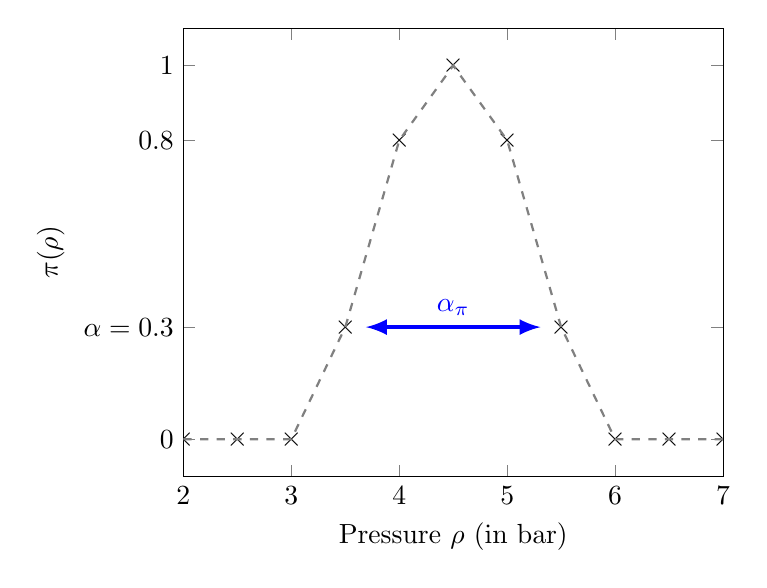
\begin{tikzpicture}[scale=1]
        \begin{axis}[%
          xlabel=Pressure $\rho$ (in bar),
          ylabel=$\pi(\rho)$,
          xmin=2, xmax=7,
          ymin=-0.1, ymax=1.1,
          ytick={0, 0.3, 0.8, 1},
          yticklabels={$0$, $\alpha=0.3$, 0.8, $1$},
          ],
          \node (a) at (2, 0) {$\times$};
          \node (b) at (2.5, 0) {$\times$};
          \node (c) at (3, 0) {$\times$};
          \node (d) at (3.5, 0.3) {$\times$};
          \node (e) at (4, 0.8) {$\times$};
          \node (f) at (4.5, 1) {$\times$};
          \node (g) at (5, 0.8) {$\times$};
          \node (h) at (5.5, 0.3) {$\times$};
          \node (i) at (6, 0) {$\times$};
          \node (j) at (6.5, 0) {$\times$};
          \node (k) at (7, 0) {$\times$};
          
          \draw [thick, dashed, gray] (a.center) -- (b.center) -- (c.center) -- (d.center) -- (e.center) -- (f.center) -- (g.center) -- (h.center) -- (i.center) -- (j.center) -- (k.center) ;
          \draw [<->, >=latex, ultra thick, blue] (d.east) -- (h.west) node [pos=0.5, above] {$\alpha_\pi$};
        \end{axis}
    \end{tikzpicture}
    \caption{Possibility distribution of \Cref{ex:bicycle_pressure_possibility} and one of its $\alpha$-cut in blue}
    \label{fig:possibility_distribution}
\end{figure}

\begin{remark}
    If you are familiar with fuzzy sets, you may have noticed that possibility distributions are similar to membership functions of a fuzzy set. Links between fuzzy sets and possibility measures have been explored in \cite{zadeh_fuzzy_1999}.
\end{remark}

Focal sets of necessity functions can be determined directly from the possibility distribution by looking at their \( \alpha \)-cuts. It has been proven that the core $\mathcal{C}$ (the set containing all focal sets) of a necessity function is (\cite{couso_necessity_2001}):
\begin{align*}
    \mathcal{C} =& \{\alpha_\pi~|~\alpha\in[0,1]\}\\
    =& \{ ~\{x\in\X~|~\pi(x)\geqslant\alpha\}~|~\alpha\in[0,1]~\}
\end{align*}
With the way focal sets are defined, they form a nested family of sets with regard to inclusion. Indeed, if an element of \(\X\) belongs to an \(\alpha\)-cut, then its possibility is greater than \(\alpha\) and therefore belongs to any other \(\alpha'\)-cut with a lower \(\alpha'\). For simplicity, we will assume that the focal sets \(a_1\enum a_n\) are already numbered using the inclusion order, \ie \( a_1\subset\ldots\subset a_n\). In this case, we will refer to the inclusion order as the ``natural'' order for possibility distributions.

\begin{remark}
    The fact that focal sets form a nested family of sets in the case of possibility distributions also implies that if $\X$ is finite and contains $n$ elements, then there can be \textit{at most} $n$ focal sets. For comparison, belief functions can have a maximum of $2^n-1$ focal sets (as the empty set cannot be a focal set). This means that necessity functions have fewer degrees of freedom than (some) belief functions, and thus can express fewer uncertainty structures. This drawback comes with the advantage of being more straightforward to construct, as we only need to specify the mass of $n$ focal sets (or the possibility of the $n$ elements of $\X$) instead of $2^n-1$. Indeed, when we think of a random variable like the outcome of a die, it can seem more natural for someone to specify degrees of possibility for each side separately than it is to specify degrees of plausibility for different sets of outcomes. 
    
    As such, possibility distribution have been used to model experts' opinion in domain such as water contamination \cite{bardossy_l-_1995}, soil contamination and radioactive risk assessment \cite{baudrit_comparing_2005,baudrit_representation_2005,baudrit_joint_2007} or weather forecasting \cite{le_carrer_beyond_2021}. Following the same philosophy, we will use possibility distributions in \Cref{chap:epistemic_uncertainty} to model the uncertainty of a measure of similarity between two image patches.
\end{remark}

Specifying a probability distribution often comes down to specifying the probability mass function over all atoms of the set of possible outcomes. In a way, possibility distributions are constructed the same way, as we specify the possibility (or the upper bounds) of every atom. One important difference is that the condition ``the sum of all masses must be equal to $1$'' is relaxed into a less constraining condition ``the possibility distribution must be equal to $1$ at least once''. In that respect, it is easier to construct a well-defined possibility distribution than it is to construct a well-defined probability distribution. However, the comparison stops there, as the two models does not represent the same type of uncertainty.

\begin{remark}
    Any probability distribution $P$ is a belief function $\Bel$, for which focal sets are only composed of singletons (atoms) and the mass distribution function of $\Bel$ equals the probability mass function of $P$ on atoms. However, a possibility distribution cannot model a probability distribution. Indeed, this would impose that its necessity $\Nec$ and plausibility $\Pi$ functions verify:
    \begin{align*}
        \forall A, &~\Nec(A) = \Pi(A)\\
        \Leftrightarrow&~1-\sup_{x\in A^c}\pi(x) = \sup_{x\in A}\pi(x)\\
        \Leftrightarrow&~ \sup_{x\in A}\pi(x) + \sup_{x\in A^c}\pi(x) = 1
    \end{align*}
    Consider this equation for any $x'$ verifying $\pi(x')=1$. This leads to the conclusion that any $x\neq x'$ has a possibility of $0$, implying that it is impossible for a random set or random variable to take any other value than $x'$, rendering it not-random. 
\end{remark}

\subsection{P-boxes}\label{sec:pboxes}
Another special type of belief function that is commonly used is that of \textit{probability boxes}, more commonly called p-boxes. Formally, a p-box is a pair of precise cumulative distribution functions $[\underline{F}, ~\overline{F}]$ defining lower and upper bounds on all cumulative events:

\begin{definition}[P-box]\label{def:p-box}
    Let $\X$ be the set of possible outcomes. A p-box is a pair of \acrshort{cdf}s $[\underline{F}, ~\overline{F}]$ from $\X$ to $[0, ~1]$ such that:
    \begin{equation}
    	\forall x \in \X,~\underline{F}(x) \leqslant \overline{F}(x) \label{eq:p-box}
    \end{equation}
    If $\X$ is not a subset of $\mathbb{R}$, then there must exist a total order on $\X$ to define a generalized p-box \cite{destercke_unifying_2008}. 
\end{definition}

\begin{remark}
    A probability distribution can be both determined by specifying its values on every atom or by specifying its values on cumulative events. We saw in \Cref{sec:possibilities} that possibility distributions are defined by bounds on atoms. Because p-boxes are defined by bounds on cumulative events, we could say that a p-box is the ``imprecise way'' of defining a probability using cumulative events, and a possibility distribution is the ``imprecise way'' of defining a probability using atoms.
\end{remark}

The credal set $\M$ induced by a p-box $[\underline{F}, ~\overline{F}]$ is:
\begin{align}
    \M([\underline{F}, ~\overline{F}]) = \{~ F ~|~ \forall x\in\X, ~\underline{F}(x)\leqslant F(x)\leqslant \overline{F}(x) ~\}
\end{align}

\begin{definition}[Focal sets of p-boxes]
    P-boxes are special cases of belief functions. It has been proven in \cite{destercke_unifying_2008} that focal sets of p-boxes have a specific form. Although focal sets shapes are reminiscent of possibilities' $\alpha$-cuts (see \Cref{fig:p-box}), they are a bit more complex to express formally. If $\X=\{x_1\enum x_n\}$ with $x_1\leqslant\ldots\leqslant x_n$, then focal sets $\alpha_{[\underline{F}, ~\overline{F}]}$ of $[\underline{F}, ~\overline{F}]$ are given for every $\alpha\in[0,~1]$ by the following expression:
    \begin{align}
        \alpha_{[\underline{F}, ~\overline{F}]}= \opi \overline{F}^{-1}(\alpha),~\underline{F}^{-1}(\alpha)\cli\label{eq:pbox_focal_set}
    \end{align}
    where $\opi\cdot,~\cdot\cli$ are intervals of integers, and $\overline{F}^{-1}$, $\underline{F}^{-1}$ are the respective pseudo-inverse of $\overline{F}$ and $\underline{F}$ defined for every $\alpha\in[0,1]$ by:
    \begin{align*}
        \overline{F}^{-1}(\alpha) =& \min \{x_i ~\st ~\overline{F}(x_i)\geqslant \alpha\}\\
        \underline{F}^{-1}(\alpha) =& \min \{x_i ~\st ~\underline{F}(x_i)\geqslant \alpha\}
    \end{align*}
    
    Still in \cite{destercke_unifying_2008}), it has been shown that the mass of each focal set $\opi x_i, ~x_j\cli$ equals to :
    \begin{align}
        m(\opi x_i, ~x_j\cli) = \min(\overline{F}(x_i), \underline{F}(x_j)) - \max(\overline{F}(x_{i-1}), \underline{F}(x_{j-1}))
    \end{align}
    With the convention that $\max(\overline{F}(x_{i-1}), \underline{F}(x_{j-1}))=0$ if $x_{i}$ is the first element and thus $x_{i-1}$ is ill-defined. 
\end{definition}

Because of their shape, focal sets of p-boxes can be totally ordered through the so-called lattice ordering on $\X$. It can be easily observed by looking at \Cref{fig:p-box}. If $a$ and $b$ are two focal sets of the same p-box $[\underline{F}, ~\overline{F}]$, then they are ordered as follows:
\begin{align}
    a\leqslant b \Leftrightarrow \min(a)\leqslant\min(b) \text{ and } \max(a)\leqslant \max(b)
\end{align}
As $\underline{F}\leqslant\overline{F}$, we are assured that there cannot be any case where $\min(a)<\min(b)$ and $\max(a)> \max(b)$. We can also define the order of focal sets using the definition of \Cref{eq:pbox_focal_set} for every $\alpha,~\beta\in[0,1]^2$:
\begin{align*}
    \opi\overline{F}^{-1}(\alpha), ~\underline{F}^{-1}(\alpha)\cli \leqslant \opi\overline{F}^{-1}(\beta), ~\underline{F}^{-1}(\beta)\cli \Leftrightarrow \alpha\leqslant\beta
\end{align*}

Given the shape of focal sets, there can be at most $2n-1$ of them in the set of $n$ possible outcomes. This is more degree of freedom than possibility distributions, but less than general belief functions.
\begin{remark}
    Contrary to possibility distributions that cannot equal to a single probability distribution, if a p-box $[\underline{F}, ~\overline{F}]$ verifies $\underline{F}=\overline{F}$, then its credal set is composed of a single probability distribution whose \acrshort{cdf} $F$ equals $\underline{F}$ and $\overline{F}$. P-boxes are thus generalizations of precise probability distributions.
\end{remark}

\begin{figure}[!ht]
    \centering
    \begin{tikzpicture}[scale=1]
        \begin{axis}[%
          xlabel=$x$,
          ylabel=$\CDF(x)$,
          %grid=major,
          domain=0:15,
          %legend entries={$\underline{F}$, $\overline{F}$},
          legend pos=south east,%
          ],
            \addplot[dotted, black, samples=16, mark=triangle, mark options={solid}, mark size=3pt] {cdf_erf(x, 1.5, 1.5)} node [pos=0.4, above left] {$\overline{F}$};
            \addlegendentry{$\overline{F}$}
            
            \addplot[dotted, black, samples=16, mark=square, mark options={solid}, mark size=3pt] {cdf_erf(x, 7.5, 1.5)} node [pos=0.6, below right] {$\underline{F}$};
            \addlegendentry{$\underline{F}$}
            
            \addplot[dotted, gray, samples=16, mark=+, mark options={solid, color=gray}, mark size=3pt] {cdf_erf(x, 4.5, 2)};
            \addlegendentry{$F$}
            
            \node (a) at (4, {cdf_erf(4, 1.5, 1.5)}) {};
            \node (b) at (10, {cdf_erf(10, 7.5, 1.5)}) {};
            
            \draw [<->, >=latex, ultra thick, blue] (a.east) -- (b.west) node [pos=0.5, above] {$\alpha_{[\underline{F}, ~\overline{F}]}$};
        \end{axis}
        \end{tikzpicture}
    \caption{A p-box $[\underline{F}, ~\overline{F}]$, a precise \acrshort{cdf} $F$ in its credal set, and one of its focal elements $\alpha_{[\underline{F}, ~\overline{F}]}$ in blue}
    \label{fig:p-box}
\end{figure}


\section{Dependency Models: Copulas}\label{sec:copulas}
During previous sections, we presented different models of uncertainty that will be considered throughout this thesis. When we will be aggregating and propagating uncertainty over multiple variables in \Cref{chap:joining_credal_sets,chap:propagating}, we will need to take into account the dependencies between our uncertain variables. In this section, we will present dependency models known as copulas, which are mathematical tools used to represent the dependency between multiple random variables. Copulas can represent many types of dependency, ranging from complete monotonicity to complete counter-monotonicity, including independence between variables. \Cref{sec:copula_def} will present the mathematical definition of a copula, as well as practical families of copulas and how they can model different dependencies. Finally, we present how to generate multivariate samples from a copula, which will be used in \Cref{sec:montecarlo}.

\subsection{Core Definitions and Examples}\label{sec:copula_def}
In the following, let $n\in\mathbb{N}^*$ be the number of uncertainty variables considered (either represented by random variables or random sets). We first introduce copulas, which are mapping from $[0,1]^n\rightarrow [0,1]$ verifying a number of properties, and that can model dependencies when considering \hyperref[theorem:sklar]{Sklar's Theorem}, which will be presented in this section.

\begin{definition}
     A copula is a multivariate cumulative distribution function $C:[0,1]^{n}\rightarrow [0,1]$ whose marginals follow uniform distributions on $[0,1]$. It can be interpreted as a joint cumulative distribution of $n$ random variables. For all $i\in\opi 1,n\cli $, we will refer to $u_i\in[0,1]$ as its $i$-th variable (or marginal). A copula satisfies a number of properties:
\begin{align}
    &\text{if }\exists j\in\opi 1,n\cli  \text{ \st }~u_j=0, \text{ then }C(u_1\enum u_j\enum u_n)=0\label{eq:zero_copula}\\
    &\forall i\in\opi 1,n\cli ,~C(1,1\enum1,u_i,1\enum1)=u_i\label{eq:copula_ones}\\
    &\forall (v_1\enum v_n)\in[0,1]^n \text{ \st }~\forall i\in\opi 1,n\cli ,~v_i\geqslant u_i\nonumber\\
    &\sum_{(w_1\enum w_n)\in\prod_{i=1}^n\{u_i, v_i\}}(-1)^{|\{i~|~w_i=u_i\}|}C(w_1\enum w_n)\geqslant 0\label{eq:cop_hvolume}
\end{align}
where $\prod_{i=1}^n$ is the Cartesian product of $n$ elements, meaning that $(w_1\enum w_n)\in\prod_{i=1}^n\{u_i, v_i\}$ is a tuple of $n$ elements, where each element is either $u_i$ or $v_i$. Additionally, $|\{i~|~w_i=u_i\}|$ refers to the cardinal of the set $\{i~|~w_i=u_i\}$. An interpretation of the value of \Cref{eq:cop_hvolume} is presented in the next remark.
\end{definition}

The first term in \Cref{eq:cop_hvolume} is also called H-volume or hyper-volume. It is used to compute joint probability mass assignments in the precise case (and also in the imprecise case, see \Cref{sec:joint_mass}). We will now use the following notation to refer to the $H$-volume:
\begin{eqnarray}\label{eq:hvolume}
    &&\forall i\in\opi 1,n\cli ,~\forall~0\leqslant u_i \leqslant v_i \leqslant 1,\nonumber\\
    &&H^{v_1\enum v_n}_{u_1\enum u_n}=\sum_{(w_1\enum w_n)\in\prod_{i=1}^n\{u_i, v_i\}}(-1)^{|\{i~|~w_i=u_i\}|}C(w_1\enum w_n)
\end{eqnarray}

\begin{remark}
    The formula of the H-volume actually represents the probability that $n$-uniform random variables are in the hyper rectangle $[u_1,v_1]\tdt[u_n,v_n]$. However, it is difficult to see this interpretation in the general case just by looking at the formula. For simplicity, consider the two-dimensional case. Using the interpretation of a copula $C$ as a \acrshort{cdf}, we can image two random uniform variables $U_1$ and $U_2$ on $[0,1]$ for which $C$ is their \acrshort{cdf}s. We thus have for all $(u_1,u_2)\in[0,1]^2$:
    \begin{equation*}
        P(U_1\leqslant u_1, U_2\leqslant u_2) = C(u_1, u_2)
    \end{equation*}
    Let $(u_1,u_2)\in[0,1]^2$ and $(v_1,v_2)\in[0,1]^2$ \st $u_1\leqslant v_1$ and $u_2\leqslant v_2$. 
    Computing the H-volume of $C$ between $(v_1,v_2)$ and $(u_1,u_2)$ yields:
    \begin{align}
        H^{v_1,v_2}_{u_1,u_2} =& ~C(v_1, v_2) - C(v_1, u_2) - C(u_1, v_2) + C(u_1, u_2)\nonumber\\
        =&~ P(U_1\leqslant v_1, ~U_2\leqslant v_2) - P(U_1\leqslant v_1, ~U_2\leqslant u_2)\nonumber\\
        &- P(U_1\leqslant u_1, ~U_2\leqslant v_2) + P(U_1\leqslant u_1, ~U_2\leqslant u_2)\nonumber\\
        =&~ P(U_1\leqslant v_1, ~u_2 < U_2 \leqslant v_2) - P(U_1\leqslant u_1, ~u_2 < U_2\leqslant v_2)\nonumber\\
        =&~ P(u_1 < U_1\leqslant v_1, ~u_2 < U_2\leqslant v_2)\label{eq:hvol_link_with_proba}
    \end{align}
    
    {\centering
    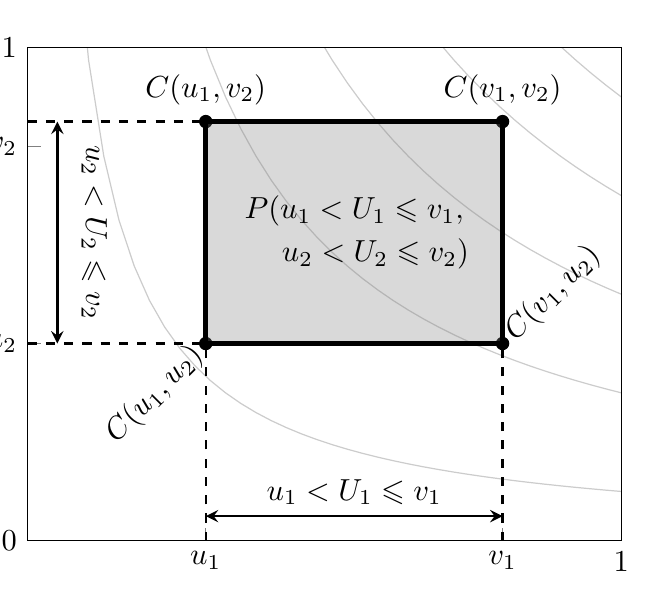
\begin{tikzpicture}[trim axis left, trim axis right, scale=1.1]
        \begin{axis}[%
            xmin=0, xmax=1,
            ymin=0, ymax=1,
            xtick={0.3, 0.8, 1},
            xticklabels={$u_1$, $v_1$, $1$},
            ytick={0, 0.4, 0.8, 1},
            yticklabels={$0$, $u_2$, $v_2$, $1$},
            xtick pos=left,
            ytick pos=left],
            
            \addplot[domain=0:1,samples=40,opacity=0.2]({x},{0.1/x});
            \addplot[domain=0:1,samples=40,opacity=0.2]({x},{0.3/x});
            \addplot[domain=0:1,samples=40,opacity=0.2]({x},{0.5/x});
            \addplot[domain=0:1,samples=40,opacity=0.2]({x},{0.7/x});
            \addplot[domain=0:1,samples=40,opacity=0.2]({x},{0.9/x});
            
            \node (a) at (0.8, 0.85) {};
            \filldraw[black] (a.center) circle (2pt) node[anchor=south,yshift=2pt]{$C(v_1,v_2)$};
            
            \node (b) at (0.3, 0.85) {};
            \filldraw[black] (b.center) circle (2pt) node[anchor=south,yshift=2pt]{$C(u_1,v_2)$};
            
            \node (c) at (0.3, 0.4) {};
            \filldraw[black] (c.center) circle (2pt) node[anchor=east,rotate=45]{$C(u_1,u_2)$};
            
            \node (d) at (0.8, 0.4) {};
            \filldraw[black] (d.center) circle (2pt) node[anchor=west, rotate=45]{$C(v_1,u_2)$};
            
            \draw[ultra thick, black, fill=gray, opacity=0.3] (c.center) rectangle (a.center);
            \draw[ultra thick, black] (c.center) rectangle (a.center) node[pos=0.5,yshift=7pt]{$P(u_1<U_1\leqslant v_1,$} node[pos=0.5, yshift=-7pt, xshift=7pt]{$u_2<U_2\leqslant v_2)$};
            
            \node (e) at (0, 0.85) {};
            \node (f) at (0, 0.4) {};
            \node (g) at (0.8, 0) {};
            \node (h) at (0.3, 0) {};
            \draw[thick, dashed, black] (e.center) -- (b.center);
            \draw[thick, dashed, black] (f.center) -- (c.center);
            \draw[thick, dashed, black] (g.center) -- (d.center);
            \draw[thick, dashed, black] (h.center) -- (c.center);
            
            \node (m) at (0.3, 0.05) {};
            \node (n) at (0.8, 0.05) {};
            \node (o) at (0.05, 0.85) {};
            \node (p) at (0.05, 0.4) {};
            
            \draw [stealth-stealth, thick, black] (m.center) -- (n.center) node[pos=0.5, above]{$u_1<U_1\leqslant v_1$};
            \draw [stealth-stealth, thick, black] (o.center) -- (p.center) node[pos=0.5, anchor=north, rotate=-90, yshift=20pt]{$u_2<U_2\leqslant v_2$};
        \end{axis}
    \end{tikzpicture}\captionof{figure}{Schematic representation of the H-volume}\par}
    
    \Cref{eq:hvol_link_with_proba} means that the H-volume represent the probability of the event
    \begin{equation*}
        u_1 < U_1\leqslant v_1, ~u_2 < U_2\leqslant v_2
    \end{equation*}
    or in other words, the probability that $(U_1, U_2)$ is in the hyper rectangle $[u_1,v_1]\times[u_2,v_2]$ (the intervals can be open or closed in the continuous case, the probability remains the same). Verifying this result for the $n$-dimensional case can be done similarly. \Cref{ex:hvolume} illustrates how the H-volume can be used to compute the discrete joint mass distribution function in the two-dimensional case. 
\end{remark}

A central theorem regarding copulas is \hyperref[theorem:sklar]{Sklar's Theorem} \cite{sklar_fonctions_1959}:
\begin{theorem}[Sklar's Theorem]\label{theorem:sklar}
    Let $F:\X_1\tdt\X_n\rightarrow[0,1]$ be a multivariate cumulative distribution function, where $\X_i\subseteq\overline{\mathbb{R}}$. The marginals $F_i$ of $F$ are defined as $\forall i\in\opi 1,n\cli , \forall x\in\X_i, F_i(x) = F( +\infty\enum  +\infty, x,  +\infty\enum +\infty)$ where $x$ is the $i$-th component of $F$. If all $F_i$ are continuous, then a unique copula $C$ exists:
    \begin{align}
        \forall (x_1\enum x_n)\in \overline{\mathbb{R}}^n, F(x_1\enum x_n)=C(F_1(x_1)\enum F_n(x_n))\label{eq:sklar_equality}
    \end{align}
    If some $F_i$ are not continuous, then $C$ is unique on the product of the ranges of all $F_i$.
    
    The reverse is also true: any copula applied to univariate cumulative distribution functions yields a multivariate cumulative distribution function whose marginals are the univariate \acrshort{cdf}s.
\end{theorem}

\hyperref[theorem:sklar]{Sklar's Theorem} thus allow to express any multivariate \acrshort{cdf} by means of its marginal \acrshort{cdf}s. Conversely, we can join multiple \acrshort{cdf}s with a copula to create a multivariate \acrshort{cdf}. A copula thus expresses the dependency between a multivariate \acrshort{cdf} and its marginals.
 
\begin{remark}
    For marginals $F_i$ that are not continuous, then there can exist multiple copula $C$ verifying \Cref{eq:sklar_equality}. However, if we note $F_i(\X_i)$ the image of $X_i$ through $F_i$, then there exists a unique copula $C$ on the ranges of images $F_1(\X_1)\tdt F_n(\X_n)$. The restriction of a copula to a subset of $I^n$ containing $0$ and $1$ is called a sub-copula. Because we work in discrete spaces, we will mostly work with sub-copulas, but the difference will be mostly transparent.
\end{remark}

Copulas are very useful to represent the dependencies between multiple uncertain variables. As such, they can play a key role in uncertainty propagation problems, explored in \Cref{chap:propagating}.

\begin{example}[Usefulness of the H-Volume]\label{ex:hvolume}
    This example will illustrate how the H-volume of a copula is used to compute the probability mass function of a multivariate probability. Let us imagine a game where a dealer throws two coins, and we are interested in the joint result of the throws. We consider the two random variables $X_1$ and $X_2$ indicating the results of each throw:
    \begin{align*}
        &X_1=0\text{ if the first coin is heads, otherwise }X_1=1\\
        &X_2=0\text{ if the second coin is heads, otherwise }X_2=1
    \end{align*}
    Let $P_1$ and $P_2$ be the probability distributions of $X_1$ and $X_2$ respectively, and assume that both heads and tails are possible outcomes for both coins. We now consider the joint probability distribution $P$ associated with the random variable $(X_1,~X_2)$, and we want to compute the probability mass distribution of $P$. We denote $F_1$, $F_2$ and $F$ the respective \acrshort{cdf}s of $P_1$, $P_2$ and $P$. With this definition, $F_1$ and $F_2$ are the marginals of $F$, and Sklar's theorem states that there exists a copula $C$ such that $F=C(F_1,~F_2)$. 
    
    The probability mass distribution of $P$ can be computed by using the H-volume. For instance, let us start by computing $P(1,1)$. By noticing the fact that:
    \begin{equation*}
        \{x\in\X~|~X_1(x)=1\}=\{x\in\X~|~F_1(X_1(x))=F_1(1)\}
    \end{equation*}
    we can write that:
    \begin{align*}
        P(X_1 = 1, X_2=1) =& ~P(F_1(X_1)= 1, F_2(X_2) = 1)\\
        =& ~P(F_1(0) < F_1(X_1)\leqslant F_1(1), ~F_2(0) < F_2(X_2)\leqslant F_2(1))
    \end{align*}
    A common result in statistics states that random variables of the form $U_1=F_1(X_1)$ and $U_2=F_2(X_2)$ are uniform on $[0,1]$. We can thus apply the result from \Cref{eq:hvol_link_with_proba}, which yields
    \begin{align*}
        P(X_1 = 1, X_2=1) =& ~P(F_1(0) < U_1 \leqslant F_1(1), ~F_2(0) < U_2 \leqslant F_2(1))\\
        =& ~H^{F_1(1),~F_2(1)}_{F_1(0),~F_2(0)}
    \end{align*}
    The probability of the atom $(1,1)$ is therefore equal to the H-volume computed between \acrshort{cdf}s $(F_1, F_2)$ at $(1, 1)$ and at $(0,0)$. Following a similar reasoning, we can compute the probability of every atom and express them as H-volumes:
    \begin{align*}
        P(X_1=0, X_2=1) =& ~H_{0, F_2(0)}^{F_1(0), F_2(1)}\\
        P(X_1=1, X_2=0) =& ~H_{F_1(0), 0}^{F_1(1), F_2(0)}\\
        P(X_1=0, X_2=0) =& ~H_{0,0}^{F_1(0), F_2(0)}
    \end{align*}
    It is possible to generalize our observation: the probability of an atom $(x_1,~\ldots,~x_n)$ is the H-volume computed between marginals \acrshort{cdf}s $(F_1,~\ldots,~F_n)$ at $(x_1,~\ldots,~x_n)$ and at the marginal atoms that precedes them. If $x_1$ is the smallest number, then the marginal \acrshort{cdf} $F_1$ before it equals $0$, \etc.
    \Cref{ex:copulas} presents numerical applications of this example with different copulas.
\end{example}

It follows from \eqref{eq:cop_hvolume} that a copula is a component-wise increasing mapping. All copulas are actually dominating and dominated by two bounds (called lower and upper Fréchet–Hoeffding bounds):
\begin{align}
    &\forall u_i \in [0,1]^n,\nonumber\\
    &\max(0, 1-n+\sum_{i=1}^n u_i) \leqslant C(u_1\enum u_n) \leqslant \min(u_1\enum u_n)
\end{align}
The upper bound is a copula, usually called the Minimum copula $C_M$. It is used to model co-monotonic variables, \ie variables for which high values occur at the same time (or similarly, where low values tend to occur simultaneously). Co-monotonicity implies a maximal covariance between variables.

The lower bound is a copula only in the case $n=2$, called the \L ukasiewicz copula $C_L(u_1,u_2)=\max(0,u_1+u_2-1)$. It is used to model counter-monotonic variables, \ie variables with a perfect negative dependence between them. This explains why the lower bound is not a copula in dimensions higher than $2$. Indeed, if $X$ has a perfect negative dependence with $Y$ and $Z$, then $Y$ and $Z$ cannot share a perfect negative dependence. However, for every $u_1\enum u_n$, there always exists a copula $C$ attaining the lower bound (which can differ for different $u_1\enum u_n$):
\begin{eqnarray*}
    \forall (u_1\enum u_n)\in[0,1]^n,~\exists C \text{ \st }~C(u_1\enum u_n) = \max(0, 1-n+\sum_{i=1}^n u_i)
\end{eqnarray*}
Independence between variables is modeled by the product copula $C_\Pi$:
\begin{equation*}
    C_\Pi(u_1\enum u_n)=\prod_{i=1}^n u_i = u_1\cdot\ldots\cdot u_n
\end{equation*}
where ``$\cdot$'' refers to the product between two scalars, as the symbol $\times$ is already used for the Cartesian product. The product copula will be used later in \Cref{subsection:product_copula}. Graphical representations of the \L ukasiewicz, product and Min copulas are displayed in \Cref{fig:copulas}. \Cref{ex:copulas} presents a setting where the Product, Minimum and \L ukasiewicz copulas are used to model dependency between random variables.

\begin{example}[Different copulas for different dependencies]\label{ex:copulas}
    Let us try to illustrate how different copulas can represent different dependencies. 
    Consider the same setting as \Cref{ex:hvolume} with two coins being thrown. For the purpose of the example, assume that the dealer throws the coins in a separate room, and comes back to tell the result. We thus never see if he is cheating or not. He only provides us this piece of information: coins seems fair when looked at separately. We therefore have the following marginals:
    \begin{eqnarray*}
    \begin{cases}
        P_1(\text{heads}) = P_1(0) = 0.5\\
        P_1(\text{tails}) = P_1(1) = 0.5\\
    \end{cases}
    \qquad\text{ and }\qquad
    \begin{cases}
        P_2(\text{heads}) = P_2(0) = 0.5\\
        P_2(\text{tails}) = P_2(1) = 0.5
    \end{cases}
    \end{eqnarray*}
    
    \begin{itemize}
        \item Assume that the dealer is not cheating and that the two coin throws are independent. In that case, the product copula $C_\Pi(u,v)=u\cdot v$ must be used to represent the independence between variables.
        Using results from the previous example, it holds that:
        \begin{align*}
            P(1,1) =& H_{F_1(1), F_2(1)}^{F_1(0), F_2(0)} = 1\cdot1 - 0.5\cdot1 - 1\cdot0.5 + 0.5\cdot0.5\\
            =& 0.25\\
            P(1,0) =& H_{F_1(0), 0}^{F_1(1), F_2(0)} = 0.25 \\
            P(0,1) =& H_{0, F_2(0)}^{F_1(0), F_2(1)} = 0.25 \\
            P(0,0) =& H_{0, 0}^{F_1(0), F_2(0)} = 0.25
        \end{align*}
        Remark that we indeed find the same results as if we directly multiplied the marginal probability mass distributions: $P(1,1) = P_1(1)\cdot P_2(1)$, \etc. We thus observe the famous result: if $P_1$ and $P_2$ are independent, then $P=P_1\cdot P_2$.
        
        \item Imagine now that the dealer is not being fair, and actually forces the second throw to land on the same side as the first one (the coins will still seem fair when looked at separately). This kind of dependency is modeled by the Minimum copula $C_M(u,v)=\min(u,v)$. In this case, the joint probability is computed as follows: 
		\begin{align*}
            P(1,1) =& H_{F_1(1), F_2(1)}^{F_1(0), F_2(0)} = \min(1,1) - \min(0.5,1) - \min(1,0.5) + \min(0.5,0.5)\\
            =& 0.5\\
            P(1,0) =& H_{F_1(0), 0}^{F_1(1), F_2(0)} =\min(1,0.5) - \min(1, 0) - \min(0.5,0.5) + \min(0,0.5)\\
            =& 0\\
            P(0,1) =& H_{0, F_2(0)}^{F_1(0), F_2(1)} = 0 \\
            P(0,0) =& H_{0, 0}^{F_1(0), F_2(0)} = \min(0.5,0.5)=0.5
        \end{align*}
        The values taken by the joint probability are now completely different from the independence case. We see that values $(0,1)$ and $(1,0)$ are indeed impossible to obtain, while $(1,1)$ and $(0,0)$ are equiprobable.
        
		\item Imagine now that the dealer is still not being fair, but this time forces the second coin to land on the first coin's opposite side. In other words, if the first coin lands on heads, then the dealer puts the second coin on tails, and inversely. Looking at marginal distributions separately will still suggest that the coins are fair. However, they appear fully counter-monotone when looked at jointly. In this case, the dependency is modeled by the \L ukasiewicz copula $C_L(u,v)=\max(0,u+v-1)$, and the joint probability equals:
		\begin{align*}
            P(1,1) =& H_{F_1(1), F_2(1)}^{F_1(0), F_2(0)} = \max(0, 1+1-1) - \max(0, 0.5+1-1)\\
            &- \max(0, 1+0.5-1) + \max(0, 0.5+0.5-1)\\
            =& 0\\
            P(1,0) =& H_{F_1(0), 0}^{F_1(1), F_2(0)} =\max(0, 1+0.5-1) - \max(0, 1+0-1)\\
            &- \max(0, 0.5+0.5-1) + \max(0, 0+0.5-1)\\
            =& 0.5\\
            P(0,1) =& H_{0, F_2(0)}^{F_1(0), F_2(1)} = 0.5 \\
            P(0,0) =& H_{0, 0}^{F_1(0), F_2(0)} = \max(0, 0.5+0.5-1)=0
        \end{align*}
        The values taken by the joint probability is now completely different than in the other cases. We see that values $(1,1)$ and $(0,0)$ are indeed impossible to obtain, while $(0,1)$ and $(1,0)$ are equiprobable.
	\end{itemize}
	Those three cases indicate how copulas can represent very different dependency structures from the same marginals. It also makes it intuitive that the \L ukasiewicz copula only allows values that are ``opposite'', whereas the Minimum copula only allows values that are similar. In those examples, the dependency is so important that knowing the result of one coin throw determines the result of the second, which is therefore modeled by extreme copulas, \ie the upper and lower Fréchet-Hoeffding bounds.  We will see in the following that there are other families of copula that allow less ``extreme'' dependencies.
\end{example}

To complete this overview of copulas, let us present other copulas that can be generated using a single parameter $\theta$ in the case $n=2$. Some famous families of copulas are presented in \Cref{tab:family_of_copula}. Those families are quite common in the literature, but this list is not exhaustive.

Another important family of copulas is the family of Gaussian copulas. Each Gaussian copula is generated with a correlation matrix $R\in[-1,1]^{(n,n)}$:
\begin{align}
    C_R(u_1\enum u_n)=\Phi_R(\Phi^{-1}(u_1)\enum \Phi^{-1}(u_n))
\end{align} where $\Phi_R$ is the joint multivariate cumulative distribution function of a Gaussian variable with correlation matrix $R$, and $\Phi^{-1}$ is the inverse cumulative distribution function of a univariate Gaussian variable. We do not know an exact form for $\Phi_R$, but we can compute it by integrating its associated Gaussian \acrshort{pdf}:
\begin{align}
   \Phi_R&(\Phi^{-1}(u_1)\enum \Phi^{-1}(u_n)) =\nonumber\\ &\int_{-\infty}^{\Phi^{-1}(u_1)}\ldots\int_{-\infty}^{\Phi^{-1}(u_n)}\frac{1}{\sqrt{(2\pi)^{n}|R|}}\exp\left(-\frac{1}{2}\begin{bmatrix}x_1 & \ldots & x_{n}\end{bmatrix}R^{-1}\begin{bmatrix}x_1 \\ \ldots \\ x_{n}\end{bmatrix}\right)dx_1\ldots dx_n
\end{align}
Where $|R|$ is the determinant of $R$. This family of copulas will be used in \Cref{sec:sources_of_uncertainty} to model the dependency between the random intensities of pixels of stereo images, for instance. 
\begin{remark}
    The product copula is actually a Gaussian copula with the identity matrix $\mathbb{I}_n$ as its covariance matrix:
    \begin{align*}
        \Phi_R&(\Phi^{-1}(u_1)\enum \Phi^{-1}(u_n)) =\\ &\int_{-\infty}^{\Phi^{-1}(u_1)}\ldots\int_{-\infty}^{\Phi^{-1}(u_n)}\frac{1}{\sqrt{(2\pi)^{n}|\mathbb{I}_n|}}\exp\left(-\frac{1}{2}\begin{bmatrix}x_1 & \ldots & x_{n}\end{bmatrix}\mathbb{I}_n^{-1}\begin{bmatrix}x_1 \\ \ldots \\ x_{n}\end{bmatrix}\right)dx_1\ldots dx_n\\
        =& \int_{-\infty}^{\Phi^{-1}(u_1)}\ldots\int_{-\infty}^{\Phi^{-1}(u_n)}\frac{1}{\sqrt{(2\pi)^{n}}}\exp(-\frac{1}{2}\sum_{i=1}^nx_i^2)dx_1\ldots dx_n\\
        =& \int_{-\infty}^{\Phi^{-1}(u_1)}\frac{1}{\sqrt{(2\pi)}}\exp(-\frac{1}{2}x_1^2)dx_1\ldots\int_{-\infty}^{\Phi^{-1}(u_n)}\frac{1}{\sqrt{(2\pi)}}\exp(-\frac{1}{2}x_n^2)dx_n\\
        =& \int_{-\infty}^{\Phi^{-1}(u_1)}\Phi'(x_1)dx_1\ldots\int_{-\infty}^{\Phi^{-1}(u_n)}\Phi'(x_n)dx_n\\
        =& ~u_1\ldots u_n
    \end{align*}
\end{remark}

\begin{figure}
    \centering
        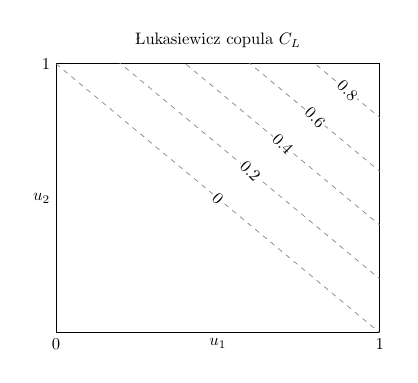
\begin{tikzpicture}[scale=0.6]
        \begin{axis}[
            xmin=0,xmax=1,
            ymin=0,ymax=1,
            xtick={0, 0.5, 1},
		    xticklabels={$0$, $u_1$, $1$},
		    ytick={0.5, 1},
		    yticklabels={$u_2$, $1$},
		    xtick style={draw=none},
		    ytick style={draw=none},
            title={\L ukasiewicz copula $C_L$},
            ]
            \addplot [domain=0:1,samples=40,style=dashed,color=gray]({x},{1-x});
            \addplot [domain=0:1,samples=40,style=dashed,color=gray]({x},{1.2-x}); 
            \addplot [domain=0:1,samples=40,style=dashed,color=gray]({x},{1.4-x}); 
            \addplot [domain=0:1,samples=40,style=dashed,color=gray]({x},{1.6-x}); 
            \addplot [domain=0:1,samples=40,style=dashed,color=gray]({x},{1.8-x});

            \node[rotate=-45, fill=white, rounded corners=2pt, inner sep=1pt] (x) at (0.5, 0.5) {0};
            \node[rotate=-45, fill=white, rounded corners=2pt, inner sep=1pt] (x) at (0.6, 0.6) {0.2};
            \node[rotate=-45, fill=white, rounded corners=2pt, inner sep=1pt] (x) at (0.7, 0.7) {0.4};
            \node[rotate=-45, fill=white, rounded corners=2pt, inner sep=1pt] (x) at (0.8, 0.8) {0.6};
            \node[rotate=-45, fill=white, rounded corners=2pt, inner sep=1pt] (x) at (0.9, 0.9) {0.8};
        \end{axis}
        \end{tikzpicture}\quad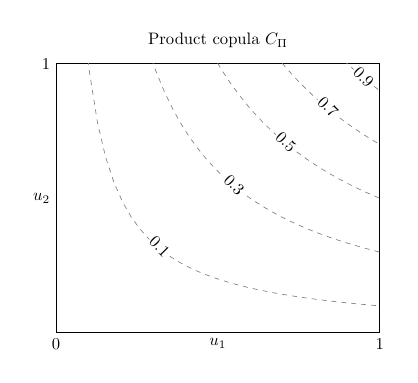
\begin{tikzpicture}[scale=0.6]
        \begin{axis}[
            xmin=0,xmax=1,
            ymin=0,ymax=1,
            xtick={0, 0.5, 1},
		    xticklabels={$0$, $u_1$, $1$},
		    ytick={0.5, 1},
		    yticklabels={$u_2$, $1$},
		    xtick style={draw=none},
		    ytick style={draw=none},
            title={Product copula $C_\Pi$},
            ]
            \addplot[domain=0:1,samples=40,style=dashed,color=gray]({x},{0.1/x});
            \addplot[domain=0:1,samples=40,style=dashed,color=gray]({x},{0.3/x}); 
            \addplot[domain=0:1,samples=40,style=dashed,color=gray]({x},{0.5/x}); 
            \addplot[domain=0:1,samples=40,style=dashed,color=gray]({x},{0.7/x}); 
            \addplot[domain=0:1,samples=40,style=dashed,color=gray]({x},{0.9/x});

            \node[rotate=-45, fill=white, rounded corners=2pt, inner sep=1pt] (x) at (0.32, 0.32) {0.1};
            \node[rotate=-45, fill=white, rounded corners=2pt, inner sep=1pt] (x) at (0.55, 0.55) {0.3};
            \node[rotate=-45, fill=white, rounded corners=2pt, inner sep=1pt] (x) at (0.71, 0.71) {0.5};
            \node[rotate=-45, fill=white, rounded corners=2pt, inner sep=1pt] (x) at (0.84, 0.84) {0.7};
            \node[rotate=-45, fill=white, rounded corners=2pt, inner sep=1pt] (x) at (0.95, 0.95) {0.9};
            
        \end{axis}
        \end{tikzpicture}\quad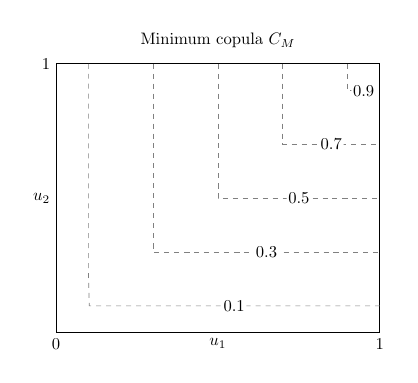
\begin{tikzpicture}[scale=0.6]
        \begin{axis}[
            xmin=0,xmax=1,
            ymin=0,ymax=1,
            xtick={0, 0.5, 1},
		    xticklabels={$0$, $u_1$, $1$},
		    ytick={0.5, 1},
		    yticklabels={$u_2$, $1$},
		    xtick style={draw=none},
		    ytick style={draw=none},
            title={Minimum copula $C_M$},
            ]
            \addplot [domain=0:1,samples=40,style=dashed,color=gray]({max(x, 0.1)},{max(1-x/0.1,0.1)});
            \addplot [domain=0:1,samples=40,style=dashed,color=gray]({max(x, 0.3)},{max(1-x/0.3,0.3)});
            \addplot [domain=0:1,samples=40,style=dashed,color=gray]({max(x, 0.5)},{max(1-x/0.5,0.5)});
            \addplot [domain=0:1,samples=40,style=dashed,color=gray]({max(x, 0.7)},{max(1-x/0.7,0.7)});
            \addplot [domain=0:1,samples=40,style=dashed,color=gray]({max(x, 0.9)},{max(1-x/0.9,0.9)});

            \node[fill=white, rounded corners=2pt, inner sep=1pt] (x) at (0.55, 0.1) {0.1};
            \node[fill=white, rounded corners=2pt, inner sep=1pt] (x) at (0.65, 0.3) {0.3};
            \node[fill=white, rounded corners=2pt, inner sep=1pt] (x) at (0.75, 0.5) {0.5};
            \node[fill=white, rounded corners=2pt, inner sep=1pt] (x) at (0.85, 0.7) {0.7};
            \node[fill=white, rounded corners=2pt, inner sep=1pt] (x) at (0.95, 0.9) {0.9};
        \end{axis}
        \end{tikzpicture}
    \caption{Bird view of the \L ukasiewicz, product and Min copulas for $n=2$. Dashed gray lines represent isolines of the copulas.}
    \label{fig:copulas}
\end{figure}


{\renewcommand{\arraystretch}{2}%
\begin{table}[!ht]
    \centering
    \begin{tabular}{|c|c|c|c|c|}
        \hline
        Family & $C(u_1,u_2)$ & $\theta \in $ & D-convex & D-concave \\
        \hline\hline
        Ali-Mikhail-Haq & $\frac{u_1u_2}{1-\theta(1-u_1)(1-u_2)}$ & $[-1,1)$ & $\theta\leqslant0$ & $\theta\geqslant 0$ \\
        \hline
        Clayton & $\left[\max(u_1^{-\theta}+u_2^{-\theta}-1,0)\right]^{-1/\theta}$ & $[-1,\infty)\backslash\{0\}$ & $\theta<0$ & $\theta>0$ \\
        \hline
        Frank & $-\frac{1}{\theta}\ln(1+\frac{(e^{-\theta u_1}-1)(e^{-\theta u_2}-1)}{e^{-\theta}-1})$ & $\mathbb{R}\backslash \{0\}$ & $\theta<0$ & $\theta>0$ \\
        \hline
        Gumbel & $u_1u_2\exp(-\theta \ln{u_1}\ln{u_2})$ & $(0,1]$ & $\theta\in(0,1]$  & Never \\
        \hline
    \end{tabular}
    \caption{Examples of families of copulas in the case $n=2$ which can be generated using a parameter \( \theta \). D-convexity/concavity is detailed in the Annex \Cref{sec:dconvexity}}
    \label{tab:family_of_copula}
\end{table}}

\begin{remark}
	As a copula is also a multivariate \acrshort{cdf}, one can imagine an ``imprecise'' copula \cite{montes_sklars_2015} similarly to what can be done with univariate probability distribution (see \Cref{sec:imprecise_probabilities}). Imprecise copulas allow modeling partially known dependencies, but can be hard to manipulate at times, as for instance the lower and upper bounds of an imprecise copula are not necessarily copulas themselves. In this thesis, we will not consider imprecise copulas.
\end{remark}

\subsection{Sampling from a Copula}\label{sec:sampling_copula}
As a copula represents the \acrshort{cdf} of a multivariate random variable, it is possible to sample from it. This section details a method for sampling from copulas in general, and a special method for sampling from Gaussian copulas. \Cref{chap:propagating} will use those methods for Monte Carlo sampling. For simplicity, let us first present a method for sampling in the case $n=2$. Given a copula $C$, and two \acrshort{cdf}s $F_X$ and $F_Y$, a method to generate a pair of observations $(x, y)$ from a joint \acrshort{cdf} $C(F_X, F_Y)$ is the following:

\begin{itemize}
    \item Sample two independent samples $u_1, u_2$ from a uniform distribution on [0,1]
    \item Set $v=\partial C^{-1}(u_2)$ where $\partial C^{-1}$ is the quasi-inverse of the partial derivative of $C$ with respect to its first variable (which exists almost everywhere and is invertible).
    \item We now have a sample $(u_1, v)$ from a multivariate random variable. Its marginals follow a uniform distribution on $[0,1]$, and its associated copula is $C$.
    \item The desired pair is $(x,y) = (F^{-1}_X(u_1), F^{-1}_Y(v))$, with $F_X^{-1}$, $F_Y^{-1}$ being the quasi-inverses of the marginals \acrshort{cdf}s.
\end{itemize}

We do not present the $n$-dimensional general case here as it is a bit more complex, but it can be found in \cite{cherubini_copula_2004}. However, drawing samples from a Gaussian $n$-copula with a correlation matrix $R$ are simpler to obtain:
\begin{itemize}
    \item Compute the Cholesky decomposition $A$ of the correlation matrix $R$
    \item Draw $n$ independent random samples $u=(u_1\enum u_n)'$ from $\mathcal{N}(0,1)$, where $\mathcal{N}$ is the normal distribution.
    \item Set $v=Au$
    \item Set $w_k=\Phi(v_k)$ where $\Phi$ is the univariate normal cumulative distribution function
    \item The desired draw is $(x_1\enum x_n)=(F^{-1}_1(w_1)\enum F^{-1}_n(w_n))$ with $F_i^{-1}$, being the quasi-inverse of the $i$-th marginal \acrshort{cdf}.
\end{itemize}

\begin{conclusion}
    In this chapter, we presented different uncertainty models, whose usage depends on the type of uncertainty and evidence available.  Choosing between the different models is often a trade-off between expressivity, compatibility and ``realism'' of the hypotheses of the considered problem. We also presented a way to combine probabilities by taking into account the dependency between random variables, using copulas. Copulas are well suited for probabilities, but their usage with \acrshort{ip} is more complex. \Cref{chap:joining_credal_sets} will investigate how \acrshort{ip} models can be combined using a copula, and \Cref{chap:propagating} will use copulas and imprecise models in a stereo matching problem.
\end{conclusion}

\clearpage

\chapter{Propagating the uncertainty of stereo images}
This chapter details the work conducted on the propagation of uncertainty from images into the cost curves of dense matching problems. We consider a simple model of uncertainty on the input images, a dependency model between the uncertain intensities of the images, and estimate the resulting uncertainty on the output cost curves. This chapter takes up work and data already published \cite{malinowski_copulas_2022, malinowski_uncertainty_2023, malinowski_robust_2024}.

\section{Sources of uncertainty in stereo matching}
\comroman{Maybe move this section after having presented the different ways to use Copulas and IP. 
Atmospheric correction, vibration, resolution of a pixel, discretization.
CO3D mission will not have the epipolar line correction problem that is encountered with pleiades images.
Epipolar line rectification for Pléiades is a problem that is not dealt here.}

To maintain simplicity in this section, we will not consider panchromatic images, such as Pléiades products, encoding the reflectance values as positive integer, usually contained in $[0, 5000]$. Instead, we consider grayscale images that have intensity levels quantified within the range $[0, 255]$, which will represent our measurable space $\X$. We hypothesize that a pixel's intensity value can deviate by no more than $1$ level from its observed value, with the observed value being the most likely. This hypothesis arises from the quantification of observed radiometric values into integers. To keep our explanation straightforward, we assume this simple hypothesis. Consequently, we model the uncertainty of each pixel $p\in I_L,I_R$ intensity with a possibility distribution $\pi$, centered around the observed intensity $i_p\in[0,255]$:
\begin{equation}
    \pi(i_p)=1,\quad \pi(i_p\pm1)=\alpha\,,
\end{equation}\label{eq:pixel_possibility}
with $\alpha \in [0,1]$. The $\pm$ indicates that both positive and negative values are considered. In our simulation, $\alpha = 0.3$ for pixels in the left image and $\alpha = 0.4$ for pixels in the right image. We use different values of $\alpha$ for the left and right images because the uncertainty model may vary between images due to differences in exposure, noise levels, or camera calibration. This model effectively states that we accept any probability distribution supported within $[i_p - 1, i_p + 1]$ where the probability measure $P$ satisfies $\{P(A) \leq \sup_{i \in A} \pi(i)\}$ as an acceptable model for our uncertainty. The mass distribution function $m_p$ associated to this credal set possesses two focal sets $a^p$:
\begin{eqnarray}
    &m_p(a^p_1=[\![i_p, i_p]\!])=1-\alpha\,\nonumber\\
    &m_p(a^p_2=[\![i_p-1, i_p + 1]\!])=\alpha\,\label{eq:pixel_mass}
\end{eqnarray}
with $[\![\cdot, \cdot]\!]$ referring to integer intervals. In particular, $[\![i_p, i_p]\!]$ correspond to the singleton $\{i_p\}$.

It is important to note that in this disparity estimation problem, we only account for the uncertainty in our input image intensities, without considering the uncertainty in our cost function's ability to correctly identify the true disparity as its minimum. In other words, we do not account for the uncertainty arising from the difference between ``two patches are very similar'' and ``the pixels at the center of the patches are homologous''. To better illustrate this, imagine a scenario where two pixels should be matched, but the surrounding patches are dissimilar. In this case, the cost function between those two patches would be high, potentially leading to the selection of a different patch with a lower cost function as the estimated disparity. The correct disparity would not be the minimum of the cost curve.

\section{Leveraging specificities to accelerate computations}
H Volume etc for SAD example, see IJAR.

\pagebreak

\chapter{Epistemic uncertainty in stereo matching}
\section{Cost functions as expert opinions}
See everything from CVPR ?
\section{Processing in areas where cost functions cannot be trusted}
Ambiguity etc
\section{Propagation in the rest of the CARS pipeline}
Rasterization and small ideas with Gabriela?
Impact of tiling : cost volume min and max is not the same from one tile to another (statistically it should be close, provided that the tile is big enough and the disparity interval is also large enough)

\pagebreak

\chapter{Results?}
\section{Monte Carlo Sampling for Cost Curves}
\section{Disparity Intervals}
\section{Ablation Studies}
\section{Elevation Confidence Intervals}
\pagebreak

\addcontentsline{toc}{chapter}{Conclusion}
\chapter*{Conclusion}
\section*{Context}
Usage of elevation data for environmental applications, urban planning, risk assessment, \etc requires the massive production of \acrfull{dsm}s. \acrshort{dsm}s at a global scale can be produced using satellites orbiting the Earth, and using different techniques such as \acrshort{lidar} measures, radar interferometry or optical photogrammetry. In particular, optical sensors, which have become relatively low-cost, allow producing dense \acrshort{dsm}s with sub-meter resolution. In this context, \acrshort{cnes} and Airbus are preparing the launch of the \acrshort{co3d} mission, consisting in two pairs of low-cost optical satellites dedicated to the production of high-resolution \acrshort{dsm}s across the globe using stereophotogrammetry.

Photogrammetry is a complex task, consisting in multiple successive algorithms to process images and extract the elevation information contained through the parallax effect. It can be divided into the following main steps:
\begin{itemize}
    \item Resampling of stereo images into a convenient geometry.
    \item Dense matching of pixels between images.
    \item Triangulation of a 3D point for each match.
    \item Rasterization of the point cloud on a regular grid.
\end{itemize}
Along these steps, many uncertainties arise, which can lead to errors of varying magnitude. The objective of this thesis was to quantify and propagate the uncertainty alongside a photogrammetry pipeline, in preparation of the \acrshort{co3d} mission. In particular, we focused on the \acrshort{cars} pipeline which will be used to process the \acrshort{co3d} data. Furthermore, one of the requirements of the \acrshort{co3d} mission is to produce a performance map alongside \acrshort{dsm}s. Many \acrshort{dsm} users also seek to know the quality of the predicted \acrshort{dsm}, usually characterized by confidence intervals. The main contribution of this thesis is precisely the development of a method for computing confidence intervals, which can also be used as a performance map for the \acrshort{co3d} mission.

\section*{Contributions}
In this thesis, we used other uncertainty models than well-known probability distributions. We considered \textit{imprecise} probabilities and more specifically possibility distributions, more adapted to model epistemic uncertainty, \ie arising from a lack of knowledge, by opposition to the uncertainty due to a purely random process. Those models define credal sets, \ie convex sets of probability distributions. 

When propagating multiple sources of uncertainty, it is required to compute a multivariate model of uncertainty accounting for the different dependencies between uncertain sources. We proposed to use dependency models known as copulas to construct multivariate credal sets. We introduced three methods for aggregating marginal credal sets into multivariate credal sets using copulas, namely $\M_{robust}$, $\M_{mass}$ and $\M_{agg}$. Those models are not equivalent, and their computation presents varying degrees of complexity. We investigated the relations between those sets depending on the copula used to join them, as well as the specific models used to define marginal credal sets, such as the aforementioned possibility distributions.

We used the previous results concerning multivariate credal sets to propagate the uncertainty in a specific part of the photogrammetry pipeline: the dense matching step. More specifically, we consider the computation of the matching cost between every pixel of the stereo images. We showed that the models could correctly estimate the propagated uncertainty regarding the matching cost on a real pair of stereo images.

The cost volume is used to compute the disparity map, encoding the pairing of pixels to be triangulated. Computing a cost volume allowing to correctly estimate the disparity is the hardest part of the stereo pipeline. Correctly estimating the uncertainty on the predicted disparity is therefore crucial for the rest of the pipeline. However, only considering the propagated uncertainty on the cost volume, as we previously did, is not sufficient for the correct uncertainty estimation of the disparity map. We therefore proposed to use possibility distributions to model the epistemic uncertainty regarding the choice of each disparity. For each considered pixel, we used those possibility distributions to determine a disparity confidence interval. We evaluated the accuracy of the intervals using real stereo images, and observed that intervals contain the true disparity at least $90\%$ of the time. This method for creating intervals can be applied to a wide range of stereo algorithms and is not restricted to satellite photogrammetry. To the best of our knowledge, it is also the first time such disparity confidence intervals are computed. 

We then propagated those disparity confidence intervals all the way to the end of the pipeline, where they take the form of elevation confidence intervals associated with the predicted \acrshort{dsm}. We evaluated the performance of elevation intervals on real satellite images, for which we possess a reference high quality \acrshort{dsm}. Intervals are once again accurate $90\%$ of the time, validating the performances of our new method. We also implemented this method for estimating disparity and elevation confidence intervals into the \acrshort{cars} (\url{https://github.com/CNES/cars}) and Pandora (\url{https://github.com/CNES/Pandora}) software, developed by \acrshort{cnes}. They are already publicly available, and can be used to produce elevation confidence intervals for \acrshort{dsm}s.

\section*{Limitations and Perspectives}
We demonstrated that possibility distributions and copulas could be used to propagate uncertainty in a problem such as the evaluation of a cost volume. Implementing this propagation remains a difficult challenge. It requires using simple cost functions and other simplifying assumptions. It also requires large processing capacities to be carried out efficiently, as we joined the uncertainty of thousands of different pixels in our experiments.

We evaluated our method for producing elevation intervals using high resolution \acrshort{dsm}s obtained from \acrshort{lidar} data. However, we only had access to \acrshort{dsm}s provided by glaciologists, or high resolution point clouds from the \acrshort{lidar} HD program. This means that we only observed landscapes which either contained glaciers, or were located in France. Extending the evaluation of intervals to a broader diversity of locations would be valuable, such as deserts or American cities.

Another limitation of our method is that it does not take into consideration the potential errors occurring \textit{before} the dense matching step. Those errors could occur when defining the epipolar geometry for instance, or on the localization model itself, for instance caused by vibration of the satellite as seen at the end of \Cref{chap:elevation_intervals}. Combining uncertainty models of the sensor itself or on its geolocation model could lead to a better estimation of the overall uncertainty of the \acrshort{dsm}. 

Different future perspective regarding our work can be considered. The method we developed for computing confidence intervals is carried out alongside the processing of the main \acrshort{dsm}, without influencing the values it contains. However, we could imagine using the information contained in the confidence intervals to facilitate or improve the different disparity or elevation predictions. Here are a few interesting leads that could be explored:
\begin{itemize}
    \item Disparity intervals could be computed a first time before any \acrshort{sgm} regularization. Then, during the \acrshort{sgm} regularization, disparities that are not contained inside disparity intervals are ignored, which could greatly reduce the amount of computation necessary. 
    \item Another approach would be to use matching cost possibilities to apply a different strategy when computing the disparity map. Currently, disparities are determined using a \textit{winner-takes-all} strategy, meaning that for each pixel, the selected disparity is the one minimizing its cost curve. We then do the same for the cost volume of the right image, and remove matches that do not verify the cross-checking test of \Cref{eq:cross-checking}. However, we could see the choice of a disparity map as a stable marriage problem \cite{irving_matching_1998}, where possibilities are interpreted as degrees of preferences. This could improve the quality of the disparity map, as the choice of each disparity would consider more information than a single cost curve. It would also provide an alternative to the \textit{winner takes all} strategy, which accounts for the vast majority of strategies used in dense matching.  
    \item We currently extend intervals in low confidence areas using quantiles computed over a set of neighboring intervals. We could consider using instead other cost functions which present better performances near depth discontinuities, or using values of the cost volume before \acrshort{sgm} regularization to better process intervals in those low confidence areas.
    \item When triangulating disparity intervals, we could take into consideration the limited resolution of line of sights. We could for instance reason with uncertain 3D volumes when computing their intersection, which would be a more realistic model than the precise lines of sight currently considered.
    \item Before the rasterization step, we could discard points for which the interval size is too large, as the potential error committed by considering this point is too high. 
    \item During rasterization, we could use information from intervals to modify the weights of each point in the final value of the \acrshort{dsm}. Points with small elevation intervals would be granted more importance in the final product than those with large intervals. 
\end{itemize}

Ideas developed in this thesis for 1D matching could be extended to 2D matching, for instance in the Pandora2D tool (\url{https://github.com/CNES/Pandora2D}). Apart from photogrammetry, ideas developed in this thesis could be used to improve confidence criteria of the alignment of image bands for multi-spectral images, for instance in the TRISHNA mission \cite{lagouarde_indo-french_2019}, or alignment of multi-temporal images, such as Sentinel-2 \cite{yan_sentinel-2a_2018}.
Taking a step back from imagery, we showed in this thesis that using other models of uncertainty than well-known probabilities can lead to new methods for estimating and characterizing potential errors. Many methods using incomplete or imperfect data for diverse applications, such as clustering, classification or decision-making, can also benefit from using imprecise probabilities.

\clearpage

\singlespace
\bibliography{thesis}

\end{document}
